\lstset{language=Java, numbers=left, numberstyle=\tiny, stepnumber=2, numbersep=5pt}
\chapter{Introduction}
\label{intro}
The following report refers to the Computer network assignment and is structured into three parts. The first part's topic is an analysis of the network protocols ICMP and IP (both v4), while the second part covers the exercises related to TCP. The final chapter describes the exercises for the new versions of ICMP and IP (v6). These exercises were done together with my lab-partner Antonio Parotta.

%%%%%%%%%%%%%%%%%%%%%%%%%%%%%%%%%%%%%%%%%%%%%%%%%%%%%%%%%%%%%%%%%%%%%%%%%%%%%%%%%%%%%%%%%%%%%%%%%%%%%%%%%
%%%%%%%%%%%%%%%%%%%%%%%%%%%%%%%%%%%%%%%%%%%%%%%%%%%%%%%%%%%%%%%%%%%%%%%%%%%%%%%%%%%%%%%%%%%%%%%%%%%%%%%%%
%%%%%%%%%%%%%%%%%%%%%%%%%%%%%%%%%%%%%%%%%%%%%%%%%%%%%%%%%%%%%%%%%%%%%%%%%%%%%%%%%%%%%%%%%%%%%%%%%%%%%%%%%
\chapter{IP/ICMP analysis}
\label{ipv4}

In this first part of the laboratory the program Wireshark was used to capture and analyse packages of different network protocols. The traffic was generated by PING-commands to send the observable packages from one lab PC to another. The following network protocols were analyzed:
\begin{itemize}
	\item Internet Protocol version 4 (IPv4)
	\item Internet Control Message Protocol version 4 (ICMPv4)
	\item Address Resolution Protocol (ARP)
	\item Carrier Sense Multiple Access/Collision Detection (CSMA/CD)
\end{itemize}
To understand how these protocols work and to be able to explain how they behave in different situations, having a look on the protocol's headers is necessary. \\\\
The PING-commands generate packages consisting of different protocol headers and transferable data. Each Ping is transformed into an Ethernet frame containing the IP and ICMP headers. Table \ref{abstract-icmp-header} is an representation of the basic ICMP Header while Table \ref{icmp-echo-request-header} shows the header for the echo request/reply packages that can be observed via Wireshark when executing the PING-commands.

\begin{table}[H]
	\centering
	\label{abstract-icmp-header}
	\begin{tabular}{|c|c|c|c|c|}
		\hline
		\textbf{bits}  & 0-7  & 8-15 & 16-23         & 24-31         \\ \hline
		\textbf{bytes} & 0    & 1    & 2             & 3             \\ \hline
		offset 0       & Type & Code & \multicolumn{2}{c|}{Checksum} \\ \hline
		offset 32      & \multicolumn{4}{c|}{Data}                   \\ \hline
	\end{tabular}
	\caption{ICMP header}
\end{table}

\begin{table}[H]
	\centering
	\label{icmp-echo-request-header}
	\begin{tabular}{|c|c|c|c|c|}
		\hline
		\textbf{bits}                   & 0-7            & 8-15           & 16-23             & 24-31            \\ \hline
		\textbf{bytes}                  & 0              & 1              & 2                 & 3                \\ \hline
		offset 0                        & Type           & Code           & \multicolumn{2}{c|}{Checksum}        \\ \hline
		\multicolumn{1}{|l|}{offset 32} & \multicolumn{2}{c|}{Identifier} & \multicolumn{2}{c|}{Sequence Number} \\ \hline
		offset 64                       & \multicolumn{4}{c|}{data}                                              \\ \hline
	\end{tabular}
	\caption{ICMP type 8 echo request/reply packet }
	
\end{table}

Table \ref{ipv4-header} shows the header for the Internet Protocol v4. Noteable here are the entered destination address as well as the source address of the sender. The Time to Live is also an important segment of the header, which will be significant later on for an specific PING-Command. IP provides the possibility to specify options for the transfered packet. This will also be used in one of the PING-Commands.

\begin{table}[H]
	\centering
	\label{ipv4-header}
	\begin{tabular}{|c|c|c|c|c|c|c|c|c|}
		\hline
		bits       & 0-3               & 4-7           & 8-11             & 12-15             & 16-18  & 19-23      & 24-27      & 28-31      \\ \hline
		bytes                            & \multicolumn{2}{c|}{0}                                              & \multicolumn{2}{c|}{1}                                               & \multicolumn{2}{c|}{2}& \multicolumn{2}{c|}{3}\\ \hline
		offset 0   & Version           & IHL           & \multicolumn{2}{c|}{Type of Service} & \multicolumn{4}{c|}{Total Length}             \\ \hline
		offset 32  & \multicolumn{4}{c|}{Identification}                                      & Flags  & \multicolumn{3}{c|}{Fragment Offset} \\ \hline
		offset 64  & \multicolumn{2}{c|}{Time to Live} & \multicolumn{2}{c|}{Protocol}        & \multicolumn{4}{c|}{Header Checksum}          \\ \hline
		offset 96  & \multicolumn{8}{c|}{Source Address}                                                                                      \\ \hline
		offset 128 & \multicolumn{8}{c|}{Destination Address}                                                                                 \\ \hline
		offset 160 & \multicolumn{8}{c|}{Options}                                                                                             \\ \hline
	\end{tabular}
	\caption{IPv4 Header}
\end{table}

Table \ref{ethernet} shows the abstract Ethernet II frame. This frame contains the MAC-addresses for source and destination, a type segment as well as the checksum for the frame. Interesting here is the Payload field. This segments contains the headers for ICMP and IP as well as the transferable data. The maximal size for this segment is 1500 bytes for one packet. But because is must contain the headers for each networking protocol (ICMP and IP), it can't be fully occupied by transferable data. This is why the Maximum Transmission Unit (MTU) is smaller. It is only 1472 bytes, because the size of the headers must be subtracted from the payload field.
$ \text{MTU } = \text{ Payload } - \text{ IP Header } - \text{ ICMP Header }$\\
$ 1500\text{ byte } - 20 \text{ byte } - 8 \text{ byte } = 1472 \text{ byte }$

\begin{table}[H]
	\centering
	\label{ethernet}
	\begin{tabular}{|l|l|l|l|l|l|}
		\hline
		Size in bit    & 24                  & 24             & 8    & 184-6000       & 16             \\ \hline
		Size in byte   & 6                   & 6              & 2    & 46 - 1500      & 4              \\ \hline
		Frame segments & Destination Address & Source Address & Type & Payload (Data) & FCS \\ \hline
	\end{tabular}
	\caption{Ethernet II frame}
\end{table}

\section{Node configuration}

Figure \ref{ip-config} shows the node configuration and settings for the computer used for the exercises in this workshop:

\begin{figure}[H]
	\centering
	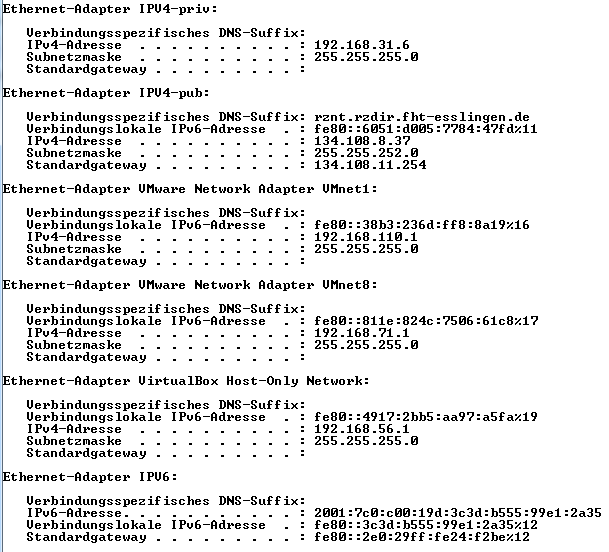
\includegraphics[width =0.7\textwidth]{ipConfig.PNG}
	\caption{Node configuration for 134.108.8.37}
	\label{ip-config}
\end{figure}

\section{Subnet internal IP Destination}
In the first exercise we created traffic by using the PING-Command to send packets to another PC within the same subnet. Figure \ref{network-internal} shows the simplified architecture for this environment:
\begin{figure}[H]
	\centering
	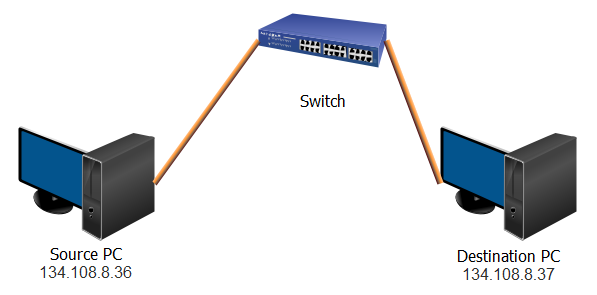
\includegraphics[width =0.7\textwidth]{Network1.PNG}
	\caption{Source and Destination PC connected with a switch in the network lab}
	\label{network-internal}
\end{figure}

\subsection{a) Basic PING command}
\label{first-ping}
The first task was sending a basic ping from one PC to another within the same subnet and capturing the sent packets using Wireshark. The PING-Command was:
\begin{center}
	\textit{ping -n 1 -l 64 134.108.8.37}
\end{center}
Listing \ref{simple-ping} shows the Wireshark trace for the captured packets. For this simple PING command, two ICMP packet were captured. One ICMP echo request was send from the source PC to the Destination PC and after this the Destination PC answers with an ICMP echo reqly. Both packets contain the Ethernet II frame as well as the IP and ICMP headers as discussed in chapter \ref{ipv4}. Each packet has the source and destination address from the IP header as well as same sequence number. The total size of each packet is 106. It contains the source and target MAC-addresses from the Ethernet frame (both 6 byte), the type of the Ethernet frame (2 byte), the IP-header (20 byte), the ICMP-header (8 byte) and the transmitted data (64 byte).

\begin{lstlisting}[caption={Wireshark trace for simple PING command},captionpos=b,label{simple-ping}]
No.     Time           Source                Destination     Protocol   Length Info
445 32.125568      134.108.8.36          134.108.8.37          ICMP     106    Echo (ping) request  id=0x0001, seq=25/6400, ttl=128 (reply in 448)

Frame 445: 106 bytes on wire (848 bits), 106 bytes captured (848 bits) on interface 0
	Interface id: 0 (\\Device\\NPF\_{55902047-E973-4FFC-B9C0-B0FAC2DA73AF})
		Interface name: \\Device\\NPF\_{55902047-E973-4FFC-B9C0-B0FAC2DA73AF}
	Encapsulation type: Ethernet (1)
	Arrival Time: Nov 17, 2017 09:46:22.558509000 Mitteleuropäische Zeit
	[Time shift for this packet: 0.000000000 seconds]
	Epoch Time: 1510908382.558509000 seconds
	[Time delta from previous captured frame: 0.000092000 seconds]
	[Time delta from previous displayed frame: 0.000000000 seconds]
	[Time since reference or first frame: 32.125568000 seconds]
	Frame Number: 445
	Frame Length: 106 bytes (848 bits)
	Capture Length: 106 bytes (848 bits)
	[Frame is marked: True]
	[Frame is ignored: False]
	[Protocols in frame: eth:ethertype:ip:icmp:data]
	[Coloring Rule Name: ICMP]
	[Coloring Rule String: icmp || icmpv6]
Ethernet II, Src: Dell\_87:b7:aa (90:b1:1c:87:b7:aa), Dst: Dell\_88:97:76 (90:b1:1c:88:97:76)
	Destination: Dell\_88:97:76 (90:b1:1c:88:97:76)
		Address: Dell\_88:97:76 (90:b1:1c:88:97:76)
		.... ..0. .... .... .... .... = LG bit: Globally unique address (factory default)
		.... ...0 .... .... .... .... = IG bit: Individual address (unicast)
	Source: Dell\_87:b7:aa (90:b1:1c:87:b7:aa)
		Address: Dell\_87:b7:aa (90:b1:1c:87:b7:aa)
		.... ..0. .... .... .... .... = LG bit: Globally unique address (factory default)
		.... ...0 .... .... .... .... = IG bit: Individual address (unicast)
	Type: IPv4 (0x0800)
Internet Protocol Version 4, Src: 134.108.8.36, Dst: 134.108.8.37
	0100 .... = Version: 4
	.... 0101 = Header Length: 20 bytes (5)
	Differentiated Services Field: 0x00 (DSCP: CS0, ECN: Not-ECT)
		0000 00.. = Differentiated Services Codepoint: Default (0)
		.... ..00 = Explicit Congestion Notification: Not ECN-Capable Transport (0)
	Total Length: 92
	Identification: 0x30fb (12539)
	Flags: 0x00
		0... .... = Reserved bit: Not set
		.0.. .... = Don´t fragment: Not set
		..0. .... = More fragments: Not set
	Fragment offset: 0
	Time to live: 128
	Protocol: ICMP (1)
	Header checksum: 0xec84 [validation disabled]
	[Header checksum status: Unverified]
	Source: 134.108.8.36
	Destination: 134.108.8.37
	[Source GeoIP: Unknown]
	[Destination GeoIP: Unknown]
Internet Control Message Protocol
	Type: 8 (Echo (ping) request)
	Code: 0
	Checksum: 0x856a [correct]
	[Checksum Status: Good]
	Identifier (BE): 1 (0x0001)
	Identifier (LE): 256 (0x0100)
	Sequence number (BE): 25 (0x0019)
	Sequence number (LE): 6400 (0x1900)
	[Response frame: 448]
	Data (64 bytes)

0000  61 62 63 64 65 66 67 68 69 6a 6b 6c 6d 6e 6f 70   abcdefghijklmnop
0010  71 72 73 74 75 76 77 61 62 63 64 65 66 67 68 69   qrstuvwabcdefghi
0020  6a 6b 6c 6d 6e 6f 70 71 72 73 74 75 76 77 61 62   jklmnopqrstuvwab
0030  63 64 65 66 67 68 69 6a 6b 6c 6d 6e 6f 70 71 72   cdefghijklmnopqr
	Data: 6162636465666768696a6b6c6d6e6f707172737475767761...
	[Length: 64]

No.     Time           Source                Destination           Protocol Length Info
448 32.125797      134.108.8.37          134.108.8.36          ICMP     106    Echo (ping) reply    id=0x0001, seq=25/6400, ttl=128 (request in 445)

Frame 448: 106 bytes on wire (848 bits), 106 bytes captured (848 bits) on interface 0
	Interface id: 0 (\\Device\\NPF\_{55902047-E973-4FFC-B9C0-B0FAC2DA73AF})
		Interface name: \\Device\\NPF\_{55902047-E973-4FFC-B9C0-B0FAC2DA73AF}
	Encapsulation type: Ethernet (1)
	Arrival Time: Nov 17, 2017 09:46:22.558738000 Mitteleuropäische Zeit
	[Time shift for this packet: 0.000000000 seconds]
	Epoch Time: 1510908382.558738000 seconds
	[Time delta from previous captured frame: 0.000005000 seconds]
	[Time delta from previous displayed frame: 0.000229000 seconds]
	[Time since reference or first frame: 32.125797000 seconds]
	Frame Number: 448
	Frame Length: 106 bytes (848 bits)
	Capture Length: 106 bytes (848 bits)
	[Frame is marked: True]
	[Frame is ignored: False]
	[Protocols in frame: eth:ethertype:ip:icmp:data]
	[Coloring Rule Name: ICMP]
	[Coloring Rule String: icmp || icmpv6]
Ethernet II, Src: Dell\_88:97:76 (90:b1:1c:88:97:76), Dst: Dell\_87:b7:aa (90:b1:1c:87:b7:aa)
	Destination: Dell\_87:b7:aa (90:b1:1c:87:b7:aa)
		Address: Dell\_87:b7:aa (90:b1:1c:87:b7:aa)
		.... ..0. .... .... .... .... = LG bit: Globally unique address (factory default)
		.... ...0 .... .... .... .... = IG bit: Individual address (unicast)
	Source: Dell\_88:97:76 (90:b1:1c:88:97:76)
		Address: Dell\_88:97:76 (90:b1:1c:88:97:76)
		.... ..0. .... .... .... .... = LG bit: Globally unique address (factory default)
		.... ...0 .... .... .... .... = IG bit: Individual address (unicast)
Type: IPv4 (0x0800)
Internet Protocol Version 4, Src: 134.108.8.37, Dst: 134.108.8.36
	0100 .... = Version: 4
	.... 0101 = Header Length: 20 bytes (5)
	Differentiated Services Field: 0x00 (DSCP: CS0, ECN: Not-ECT)
		0000 00.. = Differentiated Services Codepoint: Default (0)
		.... ..00 = Explicit Congestion Notification: Not ECN-Capable Transport (0)
	Total Length: 92
	Identification: 0x3021 (12321)
	Flags: 0x00
		0... .... = Reserved bit: Not set
		.0.. .... = Don´t fragment: Not set
		..0. .... = More fragments: Not set
	Fragment offset: 0
	Time to live: 128
	Protocol: ICMP (1)
	Header checksum: 0x0000 [validation disabled]
	[Header checksum status: Unverified]
	Source: 134.108.8.37
	Destination: 134.108.8.36
	[Source GeoIP: Unknown]
	[Destination GeoIP: Unknown]
Internet Control Message Protocol
	Type: 0 (Echo (ping) reply)
	Code: 0
	Checksum: 0x8d6a [correct]
	[Checksum Status: Good]
	Identifier (BE): 1 (0x0001)
	Identifier (LE): 256 (0x0100)
	Sequence number (BE): 25 (0x0019)
	Sequence number (LE): 6400 (0x1900)
	[Request frame: 445]
	[Response time: 0.229 ms]
	Data (64 bytes)

0000  61 62 63 64 65 66 67 68 69 6a 6b 6c 6d 6e 6f 70   abcdefghijklmnop
0010  71 72 73 74 75 76 77 61 62 63 64 65 66 67 68 69   qrstuvwabcdefghi
0020  6a 6b 6c 6d 6e 6f 70 71 72 73 74 75 76 77 61 62   jklmnopqrstuvwab
0030  63 64 65 66 67 68 69 6a 6b 6c 6d 6e 6f 70 71 72   cdefghijklmnopqr
	Data: 6162636465666768696a6b6c6d6e6f707172737475767761...
	[Length: 64]
\end{lstlisting}
\subsection{b) PING command with large data package}
For the second exercise we had to execute a PING-Command with a very large data package of 2000 byte. The PING-Command was:
\begin{center}
	\textit{ping -n 1 -l 2000 134.108.8.36}
\end{center}
Figure \ref{ping-l2000} shows the console output for this ping:
\begin{figure}[H]
	\centering
	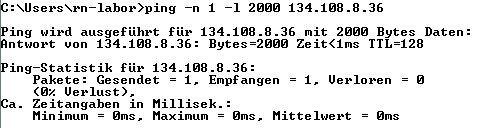
\includegraphics[width =0.7\textwidth]{ping-l200.PNG}
	\caption{Console output for PING-Command with 2000 bytes data}
	\label{ping-l2000}
\end{figure}
It seems that the protocol ICMP does not have any problems with this as the console output shows no warning. IP however does have a problem with this large packet size. As the data exceeds the Maximum Transmission Unit, the packet must be fragmented and separated into two packets. The following listing is shortened, but shows the four packages sent between both lab-PCs:
\\
\begin{lstlisting}[caption={Wireshark trace for PING command with 2000 bytes data},captionpos=b,label{l2000-ping}]
No.     Time        Source                Destination           Protocol Length DestPort Info                                                            Delta Time
236 0.000000    134.108.8.37          134.108.8.36          ICMP     1514            Echo (ping) request  id=0x0001, seq=25/6400, ttl=128 (reply in 240) 0.000000
	
Frame 236: 1514 bytes on wire (12112 bits), 1514 bytes captured (12112 bits) on interface 0
	Interface id: 0 (\\Device\\NPF\_{55902047-E973-4FFC-B9C0-B0FAC2DA73AF})
	Interface name: \\Device\\NPF\_{55902047-E973-4FFC-B9C0-B0FAC2DA73AF}
	Encapsulation type: Ethernet (1)
	Arrival Time: Nov 17, 2017 09:58:38.374317000 Mitteleuropäische Zeit
	[Time shift for this packet: 0.000000000 seconds]
	Epoch Time: 1510909118.374317000 seconds
	[Time delta from previous captured frame: 0.000024000 seconds]
	[Time delta from previous displayed frame: 0.000000000 seconds]
	[Time since reference or first frame: 36.388239000 seconds]
	Frame Number: 236
	Frame Length: 1514 bytes (12112 bits)
	Capture Length: 1514 bytes (12112 bits)
	[Frame is marked: True]
	[Frame is ignored: False]
	[Protocols in frame: eth:ethertype:ip:icmp:data]
	[Coloring Rule Name: ICMP]
	[Coloring Rule String: icmp || icmpv6]
Ethernet II, Src: 90:b1:1c:88:97:76, Dst: 90:b1:1c:87:b7:aa
	Destination: 90:b1:1c:87:b7:aa
		Address: 90:b1:1c:87:b7:aa
		.... ..0. .... .... .... .... = LG bit: Globally unique address (factory default)
		.... ...0 .... .... .... .... = IG bit: Individual address (unicast)
	Source: 90:b1:1c:88:97:76
		Address: 90:b1:1c:88:97:76
		.... ..0. .... .... .... .... = LG bit: Globally unique address (factory default)
		.... ...0 .... .... .... .... = IG bit: Individual address (unicast)
	Type: IPv4 (0x0800)
Internet Protocol Version 4, Src: 134.108.8.37, Dst: 134.108.8.36
	0100 .... = Version: 4
	.... 0101 = Header Length: 20 bytes (5)
	Differentiated Services Field: 0x00 (DSCP: CS0, ECN: Not-ECT)
	0000 00.. = Differentiated Services Codepoint: Default (0)
	.... ..00 = Explicit Congestion Notification: Not ECN-Capable Transport (0)
	Total Length: 1500
	Identification: 0x3e7e (15998)
	Flags: 0x01 (More Fragments)
		0... .... = Reserved bit: Not set
		.0.. .... = Don´t fragment: Not set
		..1. .... = More fragments: Set
	Fragment offset: 0
	Time to live: 128
	Protocol: ICMP (1)
	Header checksum: 0x0000 [validation disabled]
	[Header checksum status: Unverified]
	Source: 134.108.8.37
	Destination: 134.108.8.36
	[Source GeoIP: Unknown]
	[Destination GeoIP: Unknown]
Internet Control Message Protocol
	Type: 8 (Echo (ping) request)
	Code: 0
	Checksum: 0x7b5e [unverified] [fragmented datagram]
	[Checksum Status: Unverified]
	Identifier (BE): 1 (0x0001)
	Identifier (LE): 256 (0x0100)
	Sequence number (BE): 25 (0x0019)
	Sequence number (LE): 6400 (0x1900)
	[Response frame: 240]
	Data (1472 bytes)
		
No.     Time        Source                Destination           Protocol Length DestPort Info                                                            Delta Time
237 0.000007    134.108.8.37          134.108.8.36          IPv4     562             Fragmented IP protocol (proto=ICMP 1, off=1480, ID=3e7e)        0.000007
	
No.     Time        Source                Destination           Protocol Length DestPort Info                                                            Delta Time
240 0.000488    134.108.8.36          134.108.8.37          ICMP     1514            Echo (ping) reply    id=0x0001, seq=25/6400, ttl=128 (request in 236) 0.000488
	
No.     Time        Source                Destination           Protocol Length DestPort Info                                                            Delta Time
241 0.000002    134.108.8.36          134.108.8.37          IPv4     562             Fragmented IP protocol (proto=ICMP 1, off=1480, ID=332d)        0.000002
\end{lstlisting}

It can be observed that the first packet occupies all 1514 bytes that can be sent in one ICMP packet. Subtracting the segments from the Ethernet frame (14 byte), the IP-header (20 byte) and the ICMP-header (8 byte), there is room for 1472 byte of raw data. The remaining 528 byte of data can't be transmitted in the same packet. So the data must be fragmented and sent inside another packet. As ICMP doesn't play a role in the fragmentation, it's header isn't needed anymore in the second packet. However the second packet contains the IP-header (20 byte) as it is the protocol that manages the fragmentation and transmission controlling. The segments for the Ethernet frame (14 byte) are also included, because without that there could not be any transmission at all. So summed up the second packet has a size of 562 byte.
\subsection{c) PING command with 'don't fragment' flag}
For this last exercise another PING with 2000 byte of data was executed. But this time the 'don't fragment' flag \textbf{-f} was set:
\begin{center}
	\textit{ping -n 1 -l 2000 134.108.8.36 -f}
\end{center}
This causes a problem, because as discussed in the previous chapter this large amount of data cannot be transmitted in one single packet. So IP needs to fragment it into two separate packets. But in this case it receives the 'don't fragment' command. This contradicts the functionality of IP and it throws and error that ICMP recognizes and displays a message in the console:
\begin{figure}[H]
	\centering
	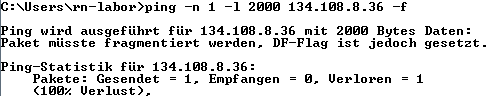
\includegraphics[width =0.7\textwidth]{ping-dontfragment.PNG}
	\caption{Console output for PING-Command with 2000 bytes data}
	\label{ping-dontfragment}
\end{figure} 
There is no Wireshark trace for this exercise, because there were no packets sent to the destination PC.
\section{Subnet external IP Destination}
For this second part of the laboratory, we moved on to PING-commands where the destination address was located in another subnet. Both subnets were connected by a router that assigned a range of addresses to the computers inside each subnet. Each computer inside one of these subnets was connected to a switch that had a connection to the router and the router provided a host IP-address for both subnets. Figure \ref{two-subnets} shows all involved network node and their IP-addresses.
\begin{figure}[H]
	\centering
	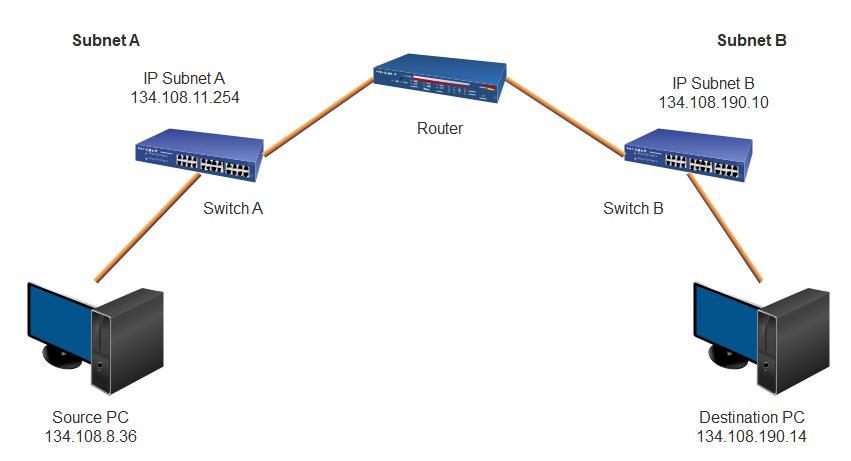
\includegraphics[width =1.0\textwidth]{two-subnets.PNG}
	\caption{Two subnets in the network lab}
	\label{two-subnets}
\end{figure} 

\subsection{d) Basic PING command with destination in another subnet}
For this exercise the following PING-Command was used:
\begin{center}
	\textit{ping -n 1 -i 2 -r 4 134.108.190.10}
\end{center}
The parameter \textbf{-r} activates the recoding of the route and sets the maximal number of records. \textbf{-i} indicates the 'Time to Live' in the IP-header (s. Chapter \ref{ipv4}) and is basically nothing more than a hop-count that decrements, when the packet passes a network node (PCs or Routers in this case). When 'Time to Live' reaches zero, the packet will be abandoned. Figure \ref{ping-subnet} shows the output of the console command:
\begin{figure}[H]
	\centering
	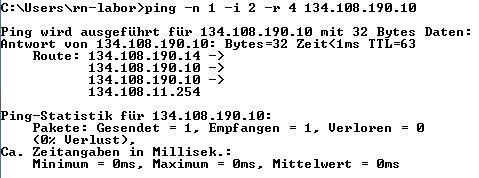
\includegraphics[width =0.7\textwidth]{ping-subnet.PNG}
	\caption{PING Command with Destination in another subnet}
	\label{ping-subnet}
\end{figure} 

The output shows the recorded route, the reply packet from the destination PC took trough the network. The sent packets are shown in the following listing:
\\
\begin{lstlisting}[caption={Wireshark trace for PING command in another subnet},captionpos=b,label{subnet-ping}]
No.     Time        Source                Destination           Protocol Length DestPort Info                                                            Delta Time
49 0.000000    134.108.8.37          134.108.190.10        ICMP     94              Echo (ping) request  id=0x0001, seq=37/9472, ttl=2 (reply in 50) 0.000000

Frame 49: 94 bytes on wire (752 bits), 94 bytes captured (752 bits) on interface 0
	Interface id: 0 (\\Device\\NPF\_{55902047-E973-4FFC-B9C0-B0FAC2DA73AF})
		Interface name: \\Device\\NPF\_{55902047-E973-4FFC-B9C0-B0FAC2DA73AF}
	Encapsulation type: Ethernet (1)
	Arrival Time: Nov 17, 2017 10:21:22.503562000 Mitteleuropäische Zeit
	[Time shift for this packet: 0.000000000 seconds]
	Epoch Time: 1510910482.503562000 seconds
	[Time delta from previous captured frame: 0.187068000 seconds]
	[Time delta from previous displayed frame: 0.000000000 seconds]
	[Time since reference or first frame: 2.480985000 seconds]
	Frame Number: 49
	Frame Length: 94 bytes (752 bits)
	Capture Length: 94 bytes (752 bits)
	[Frame is marked: True]
	[Frame is ignored: False]
	[Protocols in frame: eth:ethertype:ip:icmp:data]
	[Coloring Rule Name: ICMP]
	[Coloring Rule String: icmp || icmpv6]
	Ethernet II, Src: 90:b1:1c:88:97:76, Dst: 00:23:04:52:1c:00
	Destination: 00:23:04:52:1c:00
		Address: 00:23:04:52:1c:00
		.... ..0. .... .... .... .... = LG bit: Globally unique address (factory default)
		.... ...0 .... .... .... .... = IG bit: Individual address (unicast)
	Source: 90:b1:1c:88:97:76
		Address: 90:b1:1c:88:97:76
		.... ..0. .... .... .... .... = LG bit: Globally unique address (factory default)
		.... ...0 .... .... .... .... = IG bit: Individual address (unicast)
	Type: IPv4 (0x0800)
Internet Protocol Version 4, Src: 134.108.8.37, Dst: 134.108.190.10
	0100 .... = Version: 4
	.... 1010 = Header Length: 40 bytes (10)
	Differentiated Services Field: 0x00 (DSCP: CS0, ECN: Not-ECT)
	0000 00.. = Differentiated Services Codepoint: Default (0)
	.... ..00 = Explicit Congestion Notification: Not ECN-Capable Transport (0)
	Total Length: 80
	Identification: 0x42d5 (17109)
	Flags: 0x00
		0... .... = Reserved bit: Not set
		.0.. .... = Don´t fragment: Not set
		..0. .... = More fragments: Not set
	Fragment offset: 0
	Time to live: 2
	[Expert Info (Note/Sequence): "Time To Live" only 2]
	["Time To Live" only 2]
	[Severity level: Note]
	[Group: Sequence]
	Protocol: ICMP (1)
	Header checksum: 0x0000 [validation disabled]
	[Header checksum status: Unverified]
	Source: 134.108.8.37
	Destination: 134.108.190.10
	[Source GeoIP: Unknown]
	[Destination GeoIP: Unknown]
	Options: (20 bytes), Record Route
		IP Option - Record Route (19 bytes)
			Type: 7
			0... .... = Copy on fragmentation: No
			.00. .... = Class: Control (0)
			...0 0111 = Number: Record route (7)
			Length: 19
			Pointer: 4
			Empty Route: 0.0.0.0 <- (next)
			Empty Route: 0.0.0.0
			Empty Route: 0.0.0.0
			Empty Route: 0.0.0.0
		IP Option - End of Options List (EOL)
			Type: 0
			0... .... = Copy on fragmentation: No
			.00. .... = Class: Control (0)
			...0 0000 = Number: End of Option List (EOL) (0)
Internet Control Message Protocol
	Type: 8 (Echo (ping) request)
	Code: 0
	Checksum: 0x4d36 [correct]
	[Checksum Status: Good]
	Identifier (BE): 1 (0x0001)
	Identifier (LE): 256 (0x0100)
	Sequence number (BE): 37 (0x0025)
	Sequence number (LE): 9472 (0x2500)
	[Response frame: 50]
	Data (32 bytes)

	0000  61 62 63 64 65 66 67 68 69 6a 6b 6c 6d 6e 6f 70   abcdefghijklmnop
	0010  71 72 73 74 75 76 77 61 62 63 64 65 66 67 68 69   qrstuvwabcdefghi
	Data: 6162636465666768696a6b6c6d6e6f707172737475767761...
	Text: abcdefghijklmnopqrstuvwabcdefghi
	[Length: 32]

No.     Time        Source                Destination           Protocol Length DestPort Info                                                            Delta Time
50 0.000692    134.108.190.10        134.108.8.37          ICMP     94              Echo (ping) reply    id=0x0001, seq=37/9472, ttl=63 (request in 49) 0.000692

Frame 50: 94 bytes on wire (752 bits), 94 bytes captured (752 bits) on interface 0
	Interface id: 0 (\\Device\\NPF\_{55902047-E973-4FFC-B9C0-B0FAC2DA73AF})
		Interface name: \\Device\\NPF\_{55902047-E973-4FFC-B9C0-B0FAC2DA73AF}
	Encapsulation type: Ethernet (1)
	Arrival Time: Nov 17, 2017 10:21:22.504254000 Mitteleuropäische Zeit
	[Time shift for this packet: 0.000000000 seconds]
	Epoch Time: 1510910482.504254000 seconds
	[Time delta from previous captured frame: 0.000692000 seconds]
	[Time delta from previous displayed frame: 0.000692000 seconds]
	[Time since reference or first frame: 2.481677000 seconds]
	Frame Number: 50
	Frame Length: 94 bytes (752 bits)
	Capture Length: 94 bytes (752 bits)
	[Frame is marked: True]
	[Frame is ignored: False]
	[Protocols in frame: eth:ethertype:ip:icmp:data]
	[Coloring Rule Name: ICMP]
	[Coloring Rule String: icmp || icmpv6]
Ethernet II, Src: 00:23:04:52:1c:00, Dst: 90:b1:1c:88:97:76
	Destination: 90:b1:1c:88:97:76
		Address: 90:b1:1c:88:97:76
		.... ..0. .... .... .... .... = LG bit: Globally unique address (factory default)
		.... ...0 .... .... .... .... = IG bit: Individual address (unicast)
	Source: 00:23:04:52:1c:00
		Address: 00:23:04:52:1c:00
		.... ..0. .... .... .... .... = LG bit: Globally unique address (factory default)
		.... ...0 .... .... .... .... = IG bit: Individual address (unicast)
		Type: IPv4 (0x0800)
Internet Protocol Version 4, Src: 134.108.190.10, Dst: 134.108.8.37
	0100 .... = Version: 4
	.... 1010 = Header Length: 40 bytes (10)
	Differentiated Services Field: 0x00 (DSCP: CS0, ECN: Not-ECT)
	0000 00.. = Differentiated Services Codepoint: Default (0)
	.... ..00 = Explicit Congestion Notification: Not ECN-Capable Transport (0)
	Total Length: 80
	Identification: 0x048f (1167)
	Flags: 0x00
		0... .... = Reserved bit: Not set
		.0.. .... = Don´t fragment: Not set
		..0. .... = More fragments: Not set
	Fragment offset: 0
	Time to live: 63
	Protocol: ICMP (1)
	Header checksum: 0xafa3 [validation disabled]
	[Header checksum status: Unverified]
	Source: 134.108.190.10
	Destination: 134.108.8.37
	[Source GeoIP: Unknown]
	[Destination GeoIP: Unknown]
	Options: (20 bytes), Record Route
		IP Option - Record Route (19 bytes)
			Type: 7
			0... .... = Copy on fragmentation: No
			.00. .... = Class: Control (0)
			...0 0111 = Number: Record route (7)
			Length: 19
			Pointer: 20
			Recorded Route: 134.108.190.14
			Recorded Route: 134.108.190.10
			Recorded Route: 134.108.190.10
			Recorded Route: 134.108.11.254
		IP Option - End of Options List (EOL)
			Type: 0
			0... .... = Copy on fragmentation: No
			.00. .... = Class: Control (0)
			...0 0000 = Number: End of Option List (EOL) (0)
Internet Control Message Protocol
	Type: 0 (Echo (ping) reply)
	Code: 0
	Checksum: 0x5536 [correct]
	[Checksum Status: Good]
	Identifier (BE): 1 (0x0001)
	Identifier (LE): 256 (0x0100)
	Sequence number (BE): 37 (0x0025)
	Sequence number (LE): 9472 (0x2500)
	[Request frame: 49]
	[Response time: 0.692 ms]
	Data (32 bytes)

0000  61 62 63 64 65 66 67 68 69 6a 6b 6c 6d 6e 6f 70   abcdefghijklmnop
0010  71 72 73 74 75 76 77 61 62 63 64 65 66 67 68 69   qrstuvwabcdefghi
Data: 6162636465666768696a6b6c6d6e6f707172737475767761...
Text: abcdefghijklmnopqrstuvwabcdefghi
[Length: 32]
\end{lstlisting}
\subsection{e) PING command with reduced 'time to live'}
In this exercise the 'Time to Live' was reduced to 1 in the PING-Command:
\begin{center}
	\textit{ping -n 1 -i 1 -r 4 134.108.190.10}
\end{center}
This causes a Time-To-Live-Exceeded error that was displayed in the console output:
\begin{figure}[H]
	\centering
	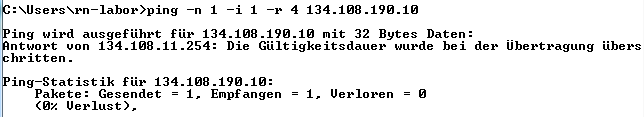
\includegraphics[width =0.8\textwidth]{ping-timetolive.PNG}
	\caption{PING Command with reduced Time to Live}
	\label{ping-timetolive}
\end{figure} 
As the 'Time to Live' is reduced to 1, it cannot reach the destination PC. When bypassing the router, the TTL is decreased to zero. So the router will drop the packet and send the Time-To-Live-Exceeded error back to the source, while the destination PC never receives any traffic. The only packet sent is from the source to the router. This can be seen in the following Wireshark trace:\\
\begin{lstlisting}[caption={Wireshark trace for PING command with reduced TTL},captionpos=b,label{timetolive-ping}]
No.     Time        Source                Destination           Protocol Length DestPort Info                                                            Delta Time
37 0.000000    134.108.8.37          134.108.190.10        ICMP     94              Echo (ping) request  id=0x0001, seq=38/9728, ttl=1 (no response found!) 0.000000

Frame 37: 94 bytes on wire (752 bits), 94 bytes captured (752 bits) on interface 0
	Interface id: 0 (\\Device\\NPF\_{55902047-E973-4FFC-B9C0-B0FAC2DA73AF})
		Interface name: \\Device\\NPF\_{55902047-E973-4FFC-B9C0-B0FAC2DA73AF}
	Encapsulation type: Ethernet (1)
	Arrival Time: Nov 17, 2017 10:23:18.619066000 Mitteleuropäische Zeit
	[Time shift for this packet: 0.000000000 seconds]
	Epoch Time: 1510910598.619066000 seconds
	[Time delta from previous captured frame: 0.145036000 seconds]
	[Time delta from previous displayed frame: 0.000000000 seconds]
	[Time since reference or first frame: 5.672194000 seconds]
	Frame Number: 37
	Frame Length: 94 bytes (752 bits)
	Capture Length: 94 bytes (752 bits)
	[Frame is marked: True]
	[Frame is ignored: False]
	[Protocols in frame: eth:ethertype:ip:icmp:data]
	[Coloring Rule Name: ICMP]
	[Coloring Rule String: icmp || icmpv6]
	Ethernet II, Src: 90:b1:1c:88:97:76, Dst: 00:23:04:52:1c:00
	Destination: 00:23:04:52:1c:00
		Address: 00:23:04:52:1c:00
		.... ..0. .... .... .... .... = LG bit: Globally unique address (factory default)
		.... ...0 .... .... .... .... = IG bit: Individual address (unicast)
	Source: 90:b1:1c:88:97:76
		Address: 90:b1:1c:88:97:76
		.... ..0. .... .... .... .... = LG bit: Globally unique address (factory default)
		.... ...0 .... .... .... .... = IG bit: Individual address (unicast)
	Type: IPv4 (0x0800)
Internet Protocol Version 4, Src: 134.108.8.37, Dst: 134.108.190.10
	0100 .... = Version: 4
	.... 1010 = Header Length: 40 bytes (10)
	Differentiated Services Field: 0x00 (DSCP: CS0, ECN: Not-ECT)
		0000 00.. = Differentiated Services Codepoint: Default (0)
		.... ..00 = Explicit Congestion Notification: Not ECN-Capable Transport (0)
	Total Length: 80
	Identification: 0x42d9 (17113)
	Flags: 0x00
		0... .... = Reserved bit: Not set
		.0.. .... = Don´t fragment: Not set
		..0. .... = More fragments: Not set
	Fragment offset: 0
	Time to live: 1
	[Expert Info (Note/Sequence): "Time To Live" only 1]
	["Time To Live" only 1]
	[Severity level: Note]
	[Group: Sequence]
	Protocol: ICMP (1)
	Header checksum: 0x0000 [validation disabled]
	[Header checksum status: Unverified]
	Source: 134.108.8.37
	Destination: 134.108.190.10
	[Source GeoIP: Unknown]
	[Destination GeoIP: Unknown]
	Options: (20 bytes), Record Route
		IP Option - Record Route (19 bytes)
			Type: 7
			0... .... = Copy on fragmentation: No
			.00. .... = Class: Control (0)
			...0 0111 = Number: Record route (7)
			Length: 19
			Pointer: 4
				Empty Route: 0.0.0.0 <- (next)
				Empty Route: 0.0.0.0
				Empty Route: 0.0.0.0
				Empty Route: 0.0.0.0
	IP Option - End of Options List (EOL)
		Type: 0
		0... .... = Copy on fragmentation: No
		.00. .... = Class: Control (0)
		...0 0000 = Number: End of Option List (EOL) (0)
Internet Control Message Protocol
	Type: 8 (Echo (ping) request)
	Code: 0
	Checksum: 0x4d35 [correct]
	[Checksum Status: Good]
	Identifier (BE): 1 (0x0001)
	Identifier (LE): 256 (0x0100)
	Sequence number (BE): 38 (0x0026)
	Sequence number (LE): 9728 (0x2600)
	[No response seen]
	[Expert Info (Warning/Sequence): No response seen to ICMP request]
	[No response seen to ICMP request]
	[Severity level: Warning]
	[Group: Sequence]
Data (32 bytes)

	0000  61 62 63 64 65 66 67 68 69 6a 6b 6c 6d 6e 6f 70   abcdefghijklmnop
	0010  71 72 73 74 75 76 77 61 62 63 64 65 66 67 68 69   qrstuvwabcdefghi
	Data: 6162636465666768696a6b6c6d6e6f707172737475767761...
	Text: abcdefghijklmnopqrstuvwabcdefghi
	[Length: 32]
\end{lstlisting}
\subsection{f) PING command with timestamps}
In this exercise the 'timestamp' option was used in the PING-Command:
\begin{center}
	\textit{ping -n 1 -i 2 -s 4 134.108.190.10}
\end{center}
The timestamp option has the effect that a timestamp which represents the amount of time from midnight to the exact moment, the packet bypasses a network node, is recorded in milliseconds:
\begin{figure}[H]
	\centering
	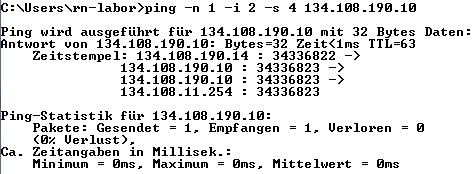
\includegraphics[width =0.8\textwidth]{ping-timestamp.PNG}
	\caption{PING Command with timestamp option}
	\label{ping-timestamp}
\end{figure} 
The time difference between the sending from the destination PC and the bypassing of the router is only 1 ms as seen in Figure \ref{ping-timestamp}. The Options Field in the IP-header contains the timestamps as seen in the following listing:
\begin{lstlisting}[caption={Wireshark trace for PING command with timestamps},captionpos=b,label{timestamp-ping}]

No.     Time        Source                Destination           Protocol Length DestPort Info                                                            Delta Time
51 0.000778    134.108.190.10        134.108.8.37          ICMP     110             Echo (ping) reply    id=0x0001, seq=43/11008, ttl=63 (request in 50) 0.000778

Frame 51: 110 bytes on wire (880 bits), 110 bytes captured (880 bits) on interface 0
	Interface id: 0 (\\Device\\NPF\_{55902047-E973-4FFC-B9C0-B0FAC2DA73AF})
		Interface name: \\Device\\NPF\_{55902047-E973-4FFC-B9C0-B0FAC2DA73AF}
	Encapsulation type: Ethernet (1)
	Arrival Time: Nov 17, 2017 10:32:16.698574000 Mitteleuropäische Zeit
	[Time shift for this packet: 0.000000000 seconds]
	Epoch Time: 1510911136.698574000 seconds
	[Time delta from previous captured frame: 0.000778000 seconds]
	[Time delta from previous displayed frame: 0.000778000 seconds]
	[Time since reference or first frame: 3.015108000 seconds]
	Frame Number: 51
	Frame Length: 110 bytes (880 bits)
	Capture Length: 110 bytes (880 bits)
	[Frame is marked: True]
	[Frame is ignored: False]
	[Protocols in frame: eth:ethertype:ip:icmp:data]
	[Coloring Rule Name: ICMP]
	[Coloring Rule String: icmp || icmpv6]
	Ethernet II, Src: 00:23:04:52:1c:00, Dst: 90:b1:1c:88:97:76
	Destination: 90:b1:1c:88:97:76
		Address: 90:b1:1c:88:97:76
		.... ..0. .... .... .... .... = LG bit: Globally unique address (factory default)
		.... ...0 .... .... .... .... = IG bit: Individual address (unicast)
	Source: 00:23:04:52:1c:00
		Address: 00:23:04:52:1c:00
		.... ..0. .... .... .... .... = LG bit: Globally unique address (factory default)
		.... ...0 .... .... .... .... = IG bit: Individual address (unicast)
	Type: IPv4 (0x0800)
Internet Protocol Version 4, Src: 134.108.190.10, Dst: 134.108.8.37
	0100 .... = Version: 4
	.... 1110 = Header Length: 56 bytes (14)
	Differentiated Services Field: 0x00 (DSCP: CS0, ECN: Not-ECT)
	0000 00.. = Differentiated Services Codepoint: Default (0)
	.... ..00 = Explicit Congestion Notification: Not ECN-Capable Transport (0)
	Total Length: 96
	Identification: 0x0490 (1168)
	Flags: 0x00
		0... .... = Reserved bit: Not set
		.0.. .... = Don´t fragment: Not set
		..0. .... = More fragments: Not set
	Fragment offset: 0
	Time to live: 63
	Protocol: ICMP (1)
	Header checksum: 0x0901 [validation disabled]
	[Header checksum status: Unverified]
	Source: 134.108.190.10
	Destination: 134.108.8.37
	[Source GeoIP: Unknown]
	[Destination GeoIP: Unknown]
	Options: (36 bytes), Time Stamp
		IP Option - Time Stamp (36 bytes)
			Type: 68
				0... .... = Copy on fragmentation: No
				.10. .... = Class: Debugging and measurement (2)
				...0 0100 = Number: Time stamp (4)
			Length: 36
			Pointer: 37
			0000 .... = Overflow: 0
			.... 0001 = Flag: Time stamp and address (0x1)
			Address: 134.108.190.14
			Time stamp: 34336822
			Address: 134.108.190.10
			Time stamp: 34336823
			Address: 134.108.190.10
			Time stamp: 34336823
			Address: 134.108.11.254
			Time stamp: 34336823
Internet Control Message Protocol
	Type: 0 (Echo (ping) reply)
	Code: 0
	Checksum: 0x5530 [correct]
	[Checksum Status: Good]
	Identifier (BE): 1 (0x0001)
	Identifier (LE): 256 (0x0100)
	Sequence number (BE): 43 (0x002b)
	Sequence number (LE): 11008 (0x2b00)
	[Request frame: 50]
	[Response time: 0.778 ms]
Data (32 bytes)

	0000  61 62 63 64 65 66 67 68 69 6a 6b 6c 6d 6e 6f 70   abcdefghijklmnop
	0010  71 72 73 74 75 76 77 61 62 63 64 65 66 67 68 69   qrstuvwabcdefghi
	Data: 6162636465666768696a6b6c6d6e6f707172737475767761...
	Text: abcdefghijklmnopqrstuvwabcdefghi
	[Length: 32]

\end{lstlisting}

\section{ARP analysis}

In the following exercises the Address Resolution Protocol was analyzed to achieve a better understanding how IP-Addresses are mapped to actual Hardware MAC-Addresses. ARP does exactly this by putting both address in relation together into a cache, also called the ARP table. Table \ref{arp-header} shows the header for ARP:
\begin{table}[H]
	\centering
	\label{arp-header}
	\begin{tabular}{|c|c|c|c|c|c|c|c|c|}
		\hline
		bits                             & \multicolumn{2}{c|}{0-7}                                                                          & \multicolumn{2}{c|}{8-15}                                                                         & \multicolumn{2}{c|}{16-23} & \multicolumn{2}{c|}{24-31} \\ \hline
		bytes                            & \multicolumn{2}{c|}{0}                                              & \multicolumn{2}{c|}{1}                                               & \multicolumn{2}{c|}{2}& \multicolumn{2}{c|}{3}\\ \hline
		Offset 0                         & \multicolumn{4}{c|}{Hardware-Addresstype (HTYPE)}                                                                                                                                                     & \multicolumn{4}{c|}{Network Protocol Type (PTYPE)}      \\ \hline
		Offset 32                        & \multicolumn{2}{c|}{\begin{tabular}[c]{@{}c@{}}Hardware \\ Address \\ Length (HLEN)\end{tabular}} & \multicolumn{2}{c|}{\begin{tabular}[c]{@{}c@{}}Protocol \\ Address \\ Length (PLEN)\end{tabular}} & \multicolumn{4}{c|}{Operation}                          \\ \hline
		Offset 64                        & \multicolumn{8}{c|}{{ Sender MAC-Address}}                                                                                                                                                                          \\ \hline
		Offset 128                       & \multicolumn{4}{c|}{{ Sender MAC-Address}}                                                                                                                & \multicolumn{4}{c|}{Sender IP Address}                  \\ \hline
		Offset 160                       & \multicolumn{4}{c|}{Sender IP Address}                                                                                                                                                                & \multicolumn{4}{c|}{Target MAC-Address}                 \\ \hline
		Offset 192                       & \multicolumn{8}{c|}{Target MAC-Address}                                                                                                                                                                                                                         \\ \hline
		\multicolumn{1}{|l|}{Offset 224} & \multicolumn{8}{c|}{Target IP-Address}                                                                                                                                                                                                                          \\ \hline
	\end{tabular}
	\caption{Address Resolution Protocol Header}
\end{table}
 
The following Figure \ref{arp-table} shows the ARP table obtained by typing 'arp -a' into the console from one of the network lab PCs before it was deleted for the next exercise:
\begin{figure}[H]
	\centering
	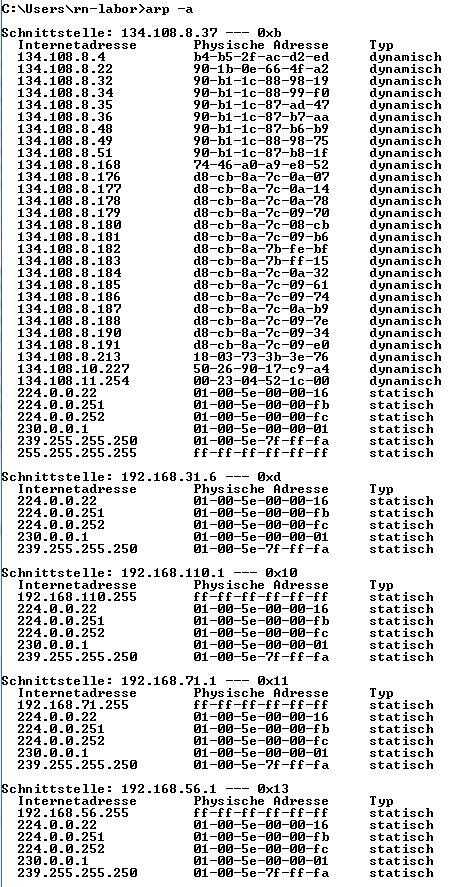
\includegraphics[width =0.7\textwidth]{urspruenglicheARPtable.PNG}
	\caption{ARP table}
	\label{arp-table}
\end{figure} 
\subsection{a) Deleting the ARP cache}
\label{apr1}
Now the ARP table on the source PC (134.108.8.37) was deleted using the console command 'arp -d'. After executing this, the ARP table was empty. After that another PING-Command was executed:\\
\begin{center}
	\textit{ping -n 2 134.108.8.36}
\end{center}
The following figure shows the output of this Ping:
\begin{figure}[H]
	\centering
	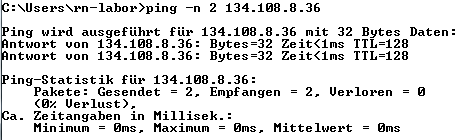
\includegraphics[width =0.8\textwidth]{ping-arp.PNG}
	\caption{PING Command Output after ARP table was deleted}
	\label{ping-arp}
\end{figure} 
Because the ARP table is now empty, IP has the problem that the target IP-Address cannot be resolved. This leads to the ARP request packet sent from the Source PC into the network via Broadcast as seen in Listing \ref{arp-ping} asking who has the required Target IP Address. The PC inside the same subnet who owns this IP Address now answers with an ARP reply packet containing it's MAC-Address. Following this the source PC inserts a new mapping with the target PC's IP- and MAC-Address into it's ARP table. After that the two PINGs are executed as seen in the following Wireshark trace:\\
\begin{lstlisting}[caption={Wireshark trace for PING command after deleting the ARP table},captionpos=b,label{arp-ping}]
No.     Time        Source                Destination           Protocol Length DestPort Info                                                            Delta Time
162 0.459379    90:b1:1c:88:97:76     ff:ff:ff:ff:ff:ff     ARP      42              Who has 134.108.8.36? Tell 134.108.8.37                         0.459379

Frame 162: 42 bytes on wire (336 bits), 42 bytes captured (336 bits) on interface 0
	Interface id: 0 (\\Device\\NPF\_{55902047-E973-4FFC-B9C0-B0FAC2DA73AF})
		Interface name: \\Device\\NPF\_{55902047-E973-4FFC-B9C0-B0FAC2DA73AF}
	Encapsulation type: Ethernet (1)
	Arrival Time: Nov 17, 2017 10:50:47.561364000 Mitteleuropäische Zeit
	[Time shift for this packet: 0.000000000 seconds]
	Epoch Time: 1510912247.561364000 seconds
	[Time delta from previous captured frame: 0.397775000 seconds]
	[Time delta from previous displayed frame: 0.459379000 seconds]
	[Time since reference or first frame: 1.803262000 seconds]
	Frame Number: 162
	Frame Length: 42 bytes (336 bits)
	Capture Length: 42 bytes (336 bits)
	[Frame is marked: True]
	[Frame is ignored: False]
	[Protocols in frame: eth:ethertype:arp]
	[Coloring Rule Name: ARP]
	[Coloring Rule String: arp]
Ethernet II, Src: 90:b1:1c:88:97:76, Dst: ff:ff:ff:ff:ff:ff
	Destination: ff:ff:ff:ff:ff:ff
		Address: ff:ff:ff:ff:ff:ff
		.... ..1. .... .... .... .... = LG bit: Locally administered address (this is NOT the factory default)
		.... ...1 .... .... .... .... = IG bit: Group address (multicast/broadcast)
	Source: 90:b1:1c:88:97:76
		Address: 90:b1:1c:88:97:76
		.... ..0. .... .... .... .... = LG bit: Globally unique address (factory default)
		.... ...0 .... .... .... .... = IG bit: Individual address (unicast)
	Type: ARP (0x0806)
Address Resolution Protocol (request)
	Hardware type: Ethernet (1)
	Protocol type: IPv4 (0x0800)
	Hardware size: 6
	Protocol size: 4
	Opcode: request (1)
	Sender MAC address: 90:b1:1c:88:97:76
	Sender IP address: 134.108.8.37
	Target MAC address: 00:00:00:00:00:00
	Target IP address: 134.108.8.36

No.     Time        Source                Destination           Protocol Length DestPort Info                                                            Delta Time
163 0.000164    90:b1:1c:87:b7:aa     90:b1:1c:88:97:76     ARP      60              134.108.8.36 is at 90:b1:1c:87:b7:aa                            0.000164

Frame 163: 60 bytes on wire (480 bits), 60 bytes captured (480 bits) on interface 0
	Interface id: 0 (\\Device\\NPF\_{55902047-E973-4FFC-B9C0-B0FAC2DA73AF})
		Interface name: \\Device\\NPF\_{55902047-E973-4FFC-B9C0-B0FAC2DA73AF}
	Encapsulation type: Ethernet (1)
	Arrival Time: Nov 17, 2017 10:50:47.561528000 Mitteleuropäische Zeit
	[Time shift for this packet: 0.000000000 seconds]
	Epoch Time: 1510912247.561528000 seconds
	[Time delta from previous captured frame: 0.000164000 seconds]
	[Time delta from previous displayed frame: 0.000164000 seconds]
	[Time since reference or first frame: 1.803426000 seconds]
	Frame Number: 163
	Frame Length: 60 bytes (480 bits)
	Capture Length: 60 bytes (480 bits)
	[Frame is marked: True]
	[Frame is ignored: False]
	[Protocols in frame: eth:ethertype:arp]
	[Coloring Rule Name: ARP]
	[Coloring Rule String: arp]
Ethernet II, Src: 90:b1:1c:87:b7:aa, Dst: 90:b1:1c:88:97:76
	Destination: 90:b1:1c:88:97:76
		Address: 90:b1:1c:88:97:76
		.... ..0. .... .... .... .... = LG bit: Globally unique address (factory default)
		.... ...0 .... .... .... .... = IG bit: Individual address (unicast)
	Source: 90:b1:1c:87:b7:aa
		Address: 90:b1:1c:87:b7:aa
		.... ..0. .... .... .... .... = LG bit: Globally unique address (factory default)
		.... ...0 .... .... .... .... = IG bit: Individual address (unicast)
	Type: ARP (0x0806)
	Padding: 000000000000000000000000000000000000
Address Resolution Protocol (reply)
	Hardware type: Ethernet (1)
	Protocol type: IPv4 (0x0800)
	Hardware size: 6
	Protocol size: 4
	Opcode: reply (2)
	Sender MAC address: 90:b1:1c:87:b7:aa
	Sender IP address: 134.108.8.36
	Target MAC address: 90:b1:1c:88:97:76
	Target IP address: 134.108.8.37

No.     Time        Source                Destination           Protocol Length DestPort Info                                                            Delta Time
164 0.000018    134.108.8.37          134.108.8.36          ICMP     74              Echo (ping) request  id=0x0001, seq=52/13312, ttl=128 (reply in 165) 0.000018


No.     Time        Source                Destination           Protocol Length DestPort Info                                                            Delta Time
165 0.000168    134.108.8.36          134.108.8.37          ICMP     74              Echo (ping) reply    id=0x0001, seq=52/13312, ttl=128 (request in 164) 0.000168


No.     Time        Source                Destination           Protocol Length DestPort Info                                                            Delta Time
176 1.005949    134.108.8.37          134.108.8.36          ICMP     74              Echo (ping) request  id=0x0001, seq=53/13568, ttl=128 (reply in 177) 1.005949


No.     Time        Source                Destination           Protocol Length DestPort Info                                                            Delta Time
177 0.000271    134.108.8.36          134.108.8.37          ICMP     74              Echo (ping) reply    id=0x0001, seq=53/13568, ttl=128 (request in 176) 0.000271

\end{lstlisting}
\subsection{b) Shutting down one PC}
For this second exercise the ARP-table on the source PC was deleted again. But this time, the target PC was shut down before the same Ping command as in \ref{arp1} was executed. The following figure \ref{ping-shutdown} shows the console output for the Ping-Command:

\begin{figure}[H]
	\centering
	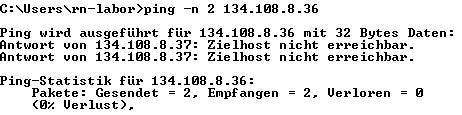
\includegraphics[width =0.8\textwidth]{ping-shutdown.PNG}
	\caption{PING Command Output after ARP table was deleted and target PC was shut down}
	\label{ping-shutdown}
\end{figure} 

Because the ARP table is empty, the source PC has to send another ARP request packet. But this time he receives no answer because the PC owning the required IP address is not reachable. The console output shows that the source PC tries to reach the target PC with another ARP request, but again there is no answer. So the communication is canceled after this. Listing \ref{label} shows the two ARP request packet that were sent from the source PC via Broadcast.\\
 \begin{lstlisting}[caption={Wireshark trace for PING command after deleting the ARP table and shutting down target PC},captionpos=b,label{arp-delete-ping}]
No.     Time           Source                Destination           Protocol Length Info
21 2.895675       Dell\_88:97:76         Broadcast             ARP      42     Who has 134.108.8.36? Tell 134.108.8.37

Frame 21: 42 bytes on wire (336 bits), 42 bytes captured (336 bits) on interface 0
Ethernet II, Src: Dell\_88:97:76 (90:b1:1c:88:97:76), Dst: Broadcast (ff:ff:ff:ff:ff:ff)
Address Resolution Protocol (request)

No.     Time           Source                Destination           Protocol Length Info
31 3.798686       Dell\_88:97:76         Broadcast             ARP      42     Who has 134.108.8.36? Tell 134.108.8.37

Frame 31: 42 bytes on wire (336 bits), 42 bytes captured (336 bits) on interface 0
Ethernet II, Src: Dell\_88:97:76 (90:b1:1c:88:97:76), Dst: Broadcast (ff:ff:ff:ff:ff:ff)
Address Resolution Protocol (request)
 \end{lstlisting}
 
\subsection{c) Reconnect after Reboot}
After rebooting the target PC and reconnecting it to the network, the same PING-Command as in \ref{apr1} was sent again from the source PC. Because now the target PC was reachable, the process and the outcome was exactly the same as in exercise \ref{apr1}.
\section{IP multicast addressing}
IP multicast addressing is used to send packets to groups of different IP addresses without broadcasting into the network. The are different protocols that are able to do this such as the Virtual Router Redundancy Protocol (VRRP), the Internet Group Management Protocol (IGMP), the routing protocol OSPF, the Network Time Protocol (NTP), the Simple Service Discovery Protocol (SSDP) and the Spanning Tree Protocol (STP). 
\\\\
The range for IP-Multicast Addresses is from 224.0.0.0 to 239.255.255.255. This can be seen when observing the intranet traffic of the Hochschule Esslingen. As a multicast packet contains a range of target IP-addresses, they cannot be exclusively mapped to a single MAC-address. So a trick is used here. The 23 lowest bits from the IP-address are put into the MAC-address. This leads to a range of MAC-addresses from 01-00-5e-00-00-00 to 01-00-5e-7f-ff-ff. The Downside is, that it is possible, that a single MAC-address can be referenced by multiple IP-Addresses. The following listing shows an SSDP packet captured from the traffic of the Hochschule Esslingen:
\begin{lstlisting}[caption={A single SSDP packet},captionpos=b,label{ssdp}]
No.     Time           Source                Destination           Protocol Length Info
4 0.461068       134.108.8.33          239.255.255.250       SSDP     175    M-SEARCH * HTTP/1.1 

Frame 4: 175 bytes on wire (1400 bits), 175 bytes captured (1400 bits) on interface 0
	Interface id: 0 (\\Device\\NPF\_{55902047-E973-4FFC-B9C0-B0FAC2DA73AF})
		Interface name: \\Device\\NPF\_{55902047-E973-4FFC-B9C0-B0FAC2DA73AF}
	Encapsulation type: Ethernet (1)
	Arrival Time: Nov 17, 2017 11:09:15.825997000 Mitteleuropäische Zeit
	[Time shift for this packet: 0.000000000 seconds]
	Epoch Time: 1510913355.825997000 seconds
	[Time delta from previous captured frame: 0.115495000 seconds]
	[Time delta from previous displayed frame: 0.115495000 seconds]
	[Time since reference or first frame: 0.461068000 seconds]
	Frame Number: 4
	Frame Length: 175 bytes (1400 bits)
	Capture Length: 175 bytes (1400 bits)
	[Frame is marked: False]
	[Frame is ignored: False]
	[Protocols in frame: eth:ethertype:ip:udp:ssdp]
	[Coloring Rule Name: UDP]
	[Coloring Rule String: udp]
	Ethernet II, Src: Dell\_87:b4:26 (90:b1:1c:87:b4:26), Dst: IPv4mcast\_7f:ff:fa (01:00:5e:7f:ff:fa)
	Destination: IPv4mcast\_7f:ff:fa (01:00:5e:7f:ff:fa)
		Address: IPv4mcast\_7f:ff:fa (01:00:5e:7f:ff:fa)
		.... ..0. .... .... .... .... = LG bit: Globally unique address (factory default)
		.... ...1 .... .... .... .... = IG bit: Group address (multicast/broadcast)
	Source: Dell\_87:b4:26 (90:b1:1c:87:b4:26)
		Address: Dell\_87:b4:26 (90:b1:1c:87:b4:26)
		.... ..0. .... .... .... .... = LG bit: Globally unique address (factory default)
		.... ...0 .... .... .... .... = IG bit: Individual address (unicast)
	Type: IPv4 (0x0800)
Internet Protocol Version 4, Src: 134.108.8.33, Dst: 239.255.255.250
	0100 .... = Version: 4
	.... 0101 = Header Length: 20 bytes (5)
	Differentiated Services Field: 0x00 (DSCP: CS0, ECN: Not-ECT)
		0000 00.. = Differentiated Services Codepoint: Default (0)
		.... ..00 = Explicit Congestion Notification: Not ECN-Capable Transport (0)
	Total Length: 161
	Identification: 0x2fc2 (12226)
	Flags: 0x00
		0... .... = Reserved bit: Not set
		.0.. .... = Don´t fragment: Not set
		..0. .... = More fragments: Not set
	Fragment offset: 0
	Time to live: 1
	Protocol: UDP (17)
	Header checksum: 0x0b03 [validation disabled]
	[Header checksum status: Unverified]
	Source: 134.108.8.33
	Destination: 239.255.255.250
	[Source GeoIP: Unknown]
	[Destination GeoIP: Unknown]
User Datagram Protocol, Src Port: 53552, Dst Port: 1900
	Source Port: 53552
	Destination Port: 1900
	Length: 141
	Checksum: 0x01c6 [unverified]
	[Checksum Status: Unverified]
	[Stream index: 0]
Simple Service Discovery Protocol
	M-SEARCH * HTTP/1.1\r\\n
		[Expert Info (Chat/Sequence): M-SEARCH * HTTP/1.1\r\\n]
			[M-SEARCH * HTTP/1.1\r\\n]
			[Severity level: Chat]
			[Group: Sequence]
		Request Method: M-SEARCH
		Request URI: *
		Request Version: HTTP/1.1
	Host:239.255.255.250:1900\r\\n
	ST:urn:schemas-upnp-org:device:InternetGatewayDevice:1\r\\n
	Man:"ssdp:discover"\r\\n
	MX:3\r\\n
	\r\\n
	[Full request URI: http://239.255.255.250:1900*]
	[HTTP request 1/19]
	[Next request in frame: 206]

\end{lstlisting}
%%%%%%%%%%%%%%%%%%%%%%%%%%%%%%%%%%%%%%%%%%%%%%%%%%%%%%%%%%%%%%%%%%%%%%%%%%%%%%%%%%%%%%%%%%%%%%%%%%%%%%%%%
%%%%%%%%%%%%%%%%%%%%%%%%%%%%%%%%%%%%%%%%%%%%%%%%%%%%%%%%%%%%%%%%%%%%%%%%%%%%%%%%%%%%%%%%%%%%%%%%%%%%%%%%%
%%%%%%%%%%%%%%%%%%%%%%%%%%%%%%%%%%%%%%%%%%%%%%%%%%%%%%%%%%%%%%%%%%%%%%%%%%%%%%%%%%%%%%%%%%%%%%%%%%%%%%%%%
\chapter{TCP analysis}
\label{tcp}
In this second part of the laboratory the Transmission Control Protocol (TCP) was examined through various exercises showing it's functionality.\\
TCP is one layer above the protocols ICMP and IP in the transport layer of the OSI-model. It's main goal is to establish a stable connection between two hosts to ensure transmission of information without data loss. Other than the protocols one layer down in the Network Layer such as ICMP or IP, TCP provides enhanced functionality for transmission control, error recovery and handling for protocol errors. These functionalities will be shown in the exercises of this laboratory. Table \ref{tcp-header} shows the TCP Header.
\begin{table}[H]
	\centering
	\label{tcp-header}
	\begin{tabular}{|c|c|c|c|c|c|c|c|c|c|c|c|c|}
		\hline
		bits       & 0-3                                                   & 4-7      & 8                                                 & 9                                                 & 10                                                & 11                                                & 12                                                & 13                                                & 14                                                & 15                                                & 16-23             & 24-31             \\ \hline
		bytes      & \multicolumn{2}{c|}{0}                                           & \multicolumn{8}{c|}{1}                                                                                                                                                                                                                                                                                                                                                                                                        & 2                 & 3                 \\ \hline
		Offset 0   & \multicolumn{10}{c|}{source port}                                                                                                                                                                                                                                                                                                                                                                                                                                                                & \multicolumn{2}{c|}{destination port} \\ \hline
		Offset 32  & \multicolumn{12}{c|}{sequence number}                                                                                                                                                                                                                                                                                                                                                                                                                                                                                                    \\ \hline
		Offset 64  & \multicolumn{12}{c|}{acknowledgment number}                                                                                                                                                                                                                                                                                                                                                                                                                                                                                             \\ \hline
		Offset 96  & \begin{tabular}[c]{@{}c@{}}data\\ offset\end{tabular} & reserved & \begin{tabular}[c]{@{}c@{}}C\\ W\\ R\end{tabular} & \begin{tabular}[c]{@{}c@{}}E\\ C\\ E\end{tabular} & \begin{tabular}[c]{@{}c@{}}U\\ R\\ G\end{tabular} & \begin{tabular}[c]{@{}c@{}}A\\ C\\ K\end{tabular} & \begin{tabular}[c]{@{}c@{}}P\\ S\\ H\end{tabular} & \begin{tabular}[c]{@{}c@{}}R\\ S\\ T\end{tabular} & \begin{tabular}[c]{@{}c@{}}S\\ Y\\ N\end{tabular} & \begin{tabular}[c]{@{}c@{}}F\\ I\\ N\end{tabular} & \multicolumn{2}{c|}{window}           \\ \hline
		Offset 128 & \multicolumn{10}{c|}{checksum}                                                                                                                                                                                                                                                                                                                                                                                                                                                                   & \multicolumn{2}{c|}{urgent pointer}   \\ \hline
		Offset 160 & \multicolumn{12}{c|}{options}                                                                                                                                                                                                                                                                                                                                                                                                                                                                                                            \\ \hline
	\end{tabular}
	\caption{Transmission Control Protocol Header}
\end{table}

TCP does not handle the networking part of the communication. This task is still handled by IP, which is one layer below TCP in the protocol stack. This is why there are no source- or target address fields in the TCP header. Instead it has segments for source- and target ports. These are necessary because a program such as \textit{Traffic}\footnote{bla} is needed for the TCP communication and these programs run on a port on both hosts. Sequence and acknowledgment numbers are used for the synchronization and error recovery between server and client. These will be important for the exercises. The control flags (each of them is only one bit) are used for traffic handling. The protocol decides how to interpret the sent data based on the set flags. They are also used for connection establishment, connection reset and for terminating a connection.

\section{Traffic generator handling}
As mentioned above, simple PING-commands weren't enough for generating traffic using the Transmission Control Protocol. A program which occupies ports on both PCs (server and client) is needed to establish a TCP connection. For this exercise a tool named \textit{Traffic} was used. The tool provides the functionality of a socket and can perform simple socket routines such as \textit{socket}, \textit{bind()}, \textit{listen()}, \textit{accept()}. It also provides a simple user interface where all functionalities are accessible for a user.

\section{Simple TCP Communication}
The first task in this laboratory was to establish a simple TCP-connection between a Server PC and a Client PC, sending multiple messages from client to server and vice versa, and finally releasing the connection.

\subsection{Connection establishment}
\label{con-est}
To establish a connection between server and client, TCP performs a routine known as the Three-Way-Handshake. The Three-Way-Handshake consists of three packets being transmitted between client and server. First, the client sends a TCP packet with the SYN-Flag containing a random number \textit{x} as sequence number (s. header in chapter \ref{tcp}) to the server. If the server is reachable, it replies with a TCP packet with the SYN and ACK-flags being enabled. Furthermore this packet contains the incremented sequence number \textit{x+1} from the client as acknowledgment number and a newly generated random number \textit{y} as sequence number. Finally the client performs the last step of the Three-Way-Handshake by replying with another ACK-flagged TCP-packet, containing the incremented sequence number from the server \textit{y+1} as acknowledgment number.\\
After these steps were successful, a stable connection is established and both client and server can begin to send data to each other. The following figure \ref{three-way-handshake} shows the steps of the Three-Way-Handshake.
\begin{figure}[H]
	\centering
	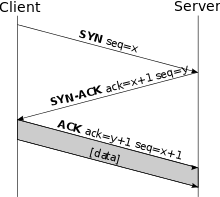
\includegraphics[width =0.4\textwidth]{Tcp-handshake.png}
	\caption{Three-Way-Handshake}
	\label{three-way-handshake}
\end{figure}
The Wireshark-trace reveals some more details about the Three-Way-Handshake. As seen in listing \ref{3way} client and server also exchange information about the Maximum Segment Size (MSS).
Furthermore both parties, the client and the server, set their window size which corresponds to
the size of the buffer. When the buffer is completely occupied with data, no more data can be transfered until the buffer is cleaned by the receiver.

\begin{lstlisting}[caption={Wireshark trace for Three-Way-Handshake},captionpos=b,label{3way}]
No.     Time           Source                Destination           Protocol Length Info
129 14.773660      134.108.8.37          134.108.8.36          TCP      66     51444 -> 6777 [SYN] Seq=0 Win=8192 Len=0 MSS=1460 WS=256 SACK\_PERM=1

Frame 129: 66 bytes on wire (528 bits), 66 bytes captured (528 bits) on interface 0
Ethernet II, Src: Dell\_88:97:76 (90:b1:1c:88:97:76), Dst: Dell\_87:b7:aa (90:b1:1c:87:b7:aa)
Internet Protocol Version 4, Src: 134.108.8.37, Dst: 134.108.8.36
Transmission Control Protocol, Src Port: 51444, Dst Port: 6777, Seq: 0, Len: 0

No.     Time           Source                Destination           Protocol Length Info
130 14.773711      134.108.8.36          134.108.8.37          TCP      66     6777 -> 51444 [SYN, ACK] Seq=0 Ack=1 Win=8192 Len=0 MSS=1460 WS=256 SACK\_PERM=1

Frame 130: 66 bytes on wire (528 bits), 66 bytes captured (528 bits) on interface 0
Ethernet II, Src: Dell\_87:b7:aa (90:b1:1c:87:b7:aa), Dst: Dell\_88:97:76 (90:b1:1c:88:97:76)
Internet Protocol Version 4, Src: 134.108.8.36, Dst: 134.108.8.37
Transmission Control Protocol, Src Port: 6777, Dst Port: 51444, Seq: 0, Ack: 1, Len: 0

No.     Time           Source                Destination           Protocol Length Info
131 14.773828      134.108.8.37          134.108.8.36          TCP      60     51444 -> 6777 [ACK] Seq=1 Ack=1 Win=65536 Len=0

Frame 131: 60 bytes on wire (480 bits), 60 bytes captured (480 bits) on interface 0
Ethernet II, Src: Dell\_88:97:76 (90:b1:1c:88:97:76), Dst: Dell\_87:b7:aa (90:b1:1c:87:b7:aa)
Internet Protocol Version 4, Src: 134.108.8.37, Dst: 134.108.8.36
Transmission Control Protocol, Src Port: 51444, Dst Port: 6777, Seq: 1, Ack: 1, Len: 0
\end{lstlisting}
\subsection{Data transfer}
After the successful establishment of the TCP connection, multiple messages were transmitted between client and server. the Wireshark trace \ref{tcp-data} shows all the packets in chronological order. All packets have in common that the PSH and ACK flags are enabled. 
\\\\
The first message was sent from client to server and contained 100 bytes of data. Because this was the first packet after the Three-Way-Handshake, both acknowledgment and sequence numbers are 1. The server answers with an ACK-packet, where the acknowledgment number is now 101. This is because the data size of the previous packet sent from client to server is added to the acknowledgment number. Also the data size is subtracted from the buffer size.
\\\\
The second message sent from client to server is much larger, containing 1000 bytes of data. The procedure is the same as for the first message. The only difference is, that the sequence number of the packet is now 101 because of the previous ACK-Packet from the server. The server answers with and ACK-packet where the acknowledgment number is now 1101. Again the data size was added here and subtracted from the buffer size of the server. The sequence number is still 1, because the server hasn't sent any data to the client yet. The window-size of the server however is now reduced to 252, because the data has not been read from the buffer yet.
\\\\
The third message follows the same procedure as message 1, but of cause this time the acknowledgment number in the server's reply packet is 1201, because there were again 100 bytes transmitted. The window size of the server is now reduced to 251.
\\\\
The last message was sent from server to client. Here the sequence number is still 1 while the acknowledgment number is already 1201. The client replies with a ACK-packet containing a acknowledgment number increased to 101, because the previous packet was the first data packet it received since the Three-Way-Handshake.

\begin{lstlisting}[caption={Wireshark trace for TCP messages},captionpos=b,label{tcp-data}]
No.     Time           Source                Destination           Protocol Length Info
41 7.691788       134.108.8.37          134.108.8.36          TCP      154    51444 -> 6777 [PSH, ACK] Seq=1 Ack=1 Win=256 Len=100

Frame 41: 154 bytes on wire (1232 bits), 154 bytes captured (1232 bits) on interface 0
Ethernet II, Src: Dell\_88:97:76 (90:b1:1c:88:97:76), Dst: Dell\_87:b7:aa (90:b1:1c:87:b7:aa)
Internet Protocol Version 4, Src: 134.108.8.37, Dst: 134.108.8.36
Transmission Control Protocol, Src Port: 51444, Dst Port: 6777, Seq: 1, Ack: 1, Len: 100
Data (100 bytes)

No.     Time           Source                Destination           Protocol Length Info
46 7.892984       134.108.8.36          134.108.8.37          TCP      54     6777 -> 51444 [ACK] Seq=1 Ack=101 Win=256 Len=0

Frame 46: 54 bytes on wire (432 bits), 54 bytes captured (432 bits) on interface 0
Ethernet II, Src: Dell\_87:b7:aa (90:b1:1c:87:b7:aa), Dst: Dell\_88:97:76 (90:b1:1c:88:97:76)
Internet Protocol Version 4, Src: 134.108.8.36, Dst: 134.108.8.37
Transmission Control Protocol, Src Port: 6777, Dst Port: 51444, Seq: 1, Ack: 101, Len: 0

No.     Time           Source                Destination           Protocol Length Info
90 19.684399      134.108.8.37          134.108.8.36          TCP      1054   51444 -> 6777 [PSH, ACK] Seq=101 Ack=1 Win=256 Len=1000

Frame 90: 1054 bytes on wire (8432 bits), 1054 bytes captured (8432 bits) on interface 0
Ethernet II, Src: Dell\_88:97:76 (90:b1:1c:88:97:76), Dst: Dell\_87:b7:aa (90:b1:1c:87:b7:aa)
Internet Protocol Version 4, Src: 134.108.8.37, Dst: 134.108.8.36
Transmission Control Protocol, Src Port: 51444, Dst Port: 6777, Seq: 101, Ack: 1, Len: 1000
Data (1000 bytes)

No.     Time           Source                Destination           Protocol Length Info
92 19.889133      134.108.8.36          134.108.8.37          TCP      54     6777 -> 51444 [ACK] Seq=1 Ack=1101 Win=252 Len=0

Frame 92: 54 bytes on wire (432 bits), 54 bytes captured (432 bits) on interface 0
Ethernet II, Src: Dell\_87:b7:aa (90:b1:1c:87:b7:aa), Dst: Dell\_88:97:76 (90:b1:1c:88:97:76)
Internet Protocol Version 4, Src: 134.108.8.36, Dst: 134.108.8.37
Transmission Control Protocol, Src Port: 6777, Dst Port: 51444, Seq: 1, Ack: 1101, Len: 0

No.     Time           Source                Destination           Protocol Length Info
1875 165.393174     134.108.8.37          134.108.8.36          TCP      154    51444 -> 6777 [PSH, ACK] Seq=1101 Ack=1 Win=256 Len=100

Frame 1875: 154 bytes on wire (1232 bits), 154 bytes captured (1232 bits) on interface 0
Ethernet II, Src: Dell\_88:97:76 (90:b1:1c:88:97:76), Dst: Dell\_87:b7:aa (90:b1:1c:87:b7:aa)
Internet Protocol Version 4, Src: 134.108.8.37, Dst: 134.108.8.36
Transmission Control Protocol, Src Port: 51444, Dst Port: 6777, Seq: 1101, Ack: 1, Len: 100
Data (100 bytes)

No.     Time           Source                Destination           Protocol Length Info
1879 165.608164     134.108.8.36          134.108.8.37          TCP      54     6777 -> 51444 [ACK] Seq=1 Ack=1201 Win=251 Len=0

Frame 1879: 54 bytes on wire (432 bits), 54 bytes captured (432 bits) on interface 0
Ethernet II, Src: Dell\_87:b7:aa (90:b1:1c:87:b7:aa), Dst: Dell\_88:97:76 (90:b1:1c:88:97:76)
Internet Protocol Version 4, Src: 134.108.8.36, Dst: 134.108.8.37
Transmission Control Protocol, Src Port: 6777, Dst Port: 51444, Seq: 1, Ack: 1201, Len: 0

No.     Time           Source                Destination           Protocol Length Info
2086 201.626400     134.108.8.36          134.108.8.37          TCP      154    6777 -> 51444 [PSH, ACK] Seq=1 Ack=1201 Win=251 Len=100

Frame 2086: 154 bytes on wire (1232 bits), 154 bytes captured (1232 bits) on interface 0
Ethernet II, Src: Dell\_87:b7:aa (90:b1:1c:87:b7:aa), Dst: Dell\_88:97:76 (90:b1:1c:88:97:76)
Internet Protocol Version 4, Src: 134.108.8.36, Dst: 134.108.8.37
Transmission Control Protocol, Src Port: 6777, Dst Port: 51444, Seq: 1, Ack: 1201, Len: 100
Data (100 bytes)

No.     Time           Source                Destination           Protocol Length Info
2088 201.832292     134.108.8.37          134.108.8.36          TCP      60     51444 -> 6777 [ACK] Seq=1201 Ack=101 Win=256 Len=0

Frame 2088: 60 bytes on wire (480 bits), 60 bytes captured (480 bits) on interface 0
Ethernet II, Src: Dell\_88:97:76 (90:b1:1c:88:97:76), Dst: Dell\_87:b7:aa (90:b1:1c:87:b7:aa)
Internet Protocol Version 4, Src: 134.108.8.37, Dst: 134.108.8.36
Transmission Control Protocol, Src Port: 51444, Dst Port: 6777, Seq: 1201, Ack: 101, Len: 0
\end{lstlisting}
\subsection{Connection release}
To terminate an active connection, one of the two connected nodes sends a TCP-packet with the FIN-Flag enabled to the other node. In this case the client releases the connection first. The server answers with an ACK-packet where the acknowledgment number is increased to 102 because of the FIN-Flag. At this point, the connection is half-closed. The server can still send data to the client, but the client cannot send any data to the server, because it already released the connection. Now the server sends a FIN-enabled TCP packet to the client to terminated it's side of the connection. The client answers with an ACK-packet where the sequence number is 102 as before and the acknowledgment number is increased from 1201 to 1202 because of the server's FIN-flag in the previous packet. Now the connection is fully terminated. The following Wireshark-trace shows the captured packets:

\begin{lstlisting}[caption={Wireshark trace for Connection Release},captionpos=b,label{tcp-fin}]
No.     Time           Source                Destination           Protocol Length Info
3752 554.875797     134.108.8.36          134.108.8.37          TCP      54     6777 -> 51444 [FIN, ACK] Seq=101 Ack=1201 Win=251 Len=0

Frame 3752: 54 bytes on wire (432 bits), 54 bytes captured (432 bits) on interface 0
Ethernet II, Src: Dell\_87:b7:aa (90:b1:1c:87:b7:aa), Dst: Dell\_88:97:76 (90:b1:1c:88:97:76)
Internet Protocol Version 4, Src: 134.108.8.36, Dst: 134.108.8.37
Transmission Control Protocol, Src Port: 6777, Dst Port: 51444, Seq: 101, Ack: 1201, Len: 0

No.     Time           Source                Destination           Protocol Length Info
3755 554.876001     134.108.8.37          134.108.8.36          TCP      60     51444 -> 6777 [ACK] Seq=1201 Ack=102 Win=256 Len=0

Frame 3755: 60 bytes on wire (480 bits), 60 bytes captured (480 bits) on interface 0
Ethernet II, Src: Dell\_88:97:76 (90:b1:1c:88:97:76), Dst: Dell\_87:b7:aa (90:b1:1c:87:b7:aa)
Internet Protocol Version 4, Src: 134.108.8.37, Dst: 134.108.8.36
Transmission Control Protocol, Src Port: 51444, Dst Port: 6777, Seq: 1201, Ack: 102, Len: 0

No.     Time           Source                Destination           Protocol Length Info
3869 569.922788     134.108.8.37          134.108.8.36          TCP      60     51444 -> 6777 [FIN, ACK] Seq=1201 Ack=102 Win=256 Len=0

Frame 3869: 60 bytes on wire (480 bits), 60 bytes captured (480 bits) on interface 0
Ethernet II, Src: Dell\_88:97:76 (90:b1:1c:88:97:76), Dst: Dell\_87:b7:aa (90:b1:1c:87:b7:aa)
Internet Protocol Version 4, Src: 134.108.8.37, Dst: 134.108.8.36
Transmission Control Protocol, Src Port: 51444, Dst Port: 6777, Seq: 1201, Ack: 102, Len: 0

No.     Time           Source                Destination           Protocol Length Info
3870 569.922807     134.108.8.36          134.108.8.37          TCP      54     6777 -> 51444 [ACK] Seq=102 Ack=1202 Win=251 Len=0

Frame 3870: 54 bytes on wire (432 bits), 54 bytes captured (432 bits) on interface 0
Ethernet II, Src: Dell\_87:b7:aa (90:b1:1c:87:b7:aa), Dst: Dell\_88:97:76 (90:b1:1c:88:97:76)
Internet Protocol Version 4, Src: 134.108.8.36, Dst: 134.108.8.37
Transmission Control Protocol, Src Port: 6777, Dst Port: 51444, Seq: 102, Ack: 1202, Len: 0

\end{lstlisting}

\section{TCP flow control}
For this exercise another connection between server and client was established the same way as before. Now the task was to send a burst of 100 message from one host to another, while each message contained 1000 bytes of data. The intention behind this is to completely occupy the server's receive buffer with data and to observe what happens next. As seen in the Wireshark-trace, the client sends packet after packet to the server until the Window-size in the Servers corresponding ACK-packet is decreased to a value beneath 1000 bytes. When the client now tries to send the next packet, the server answers with a \textbf{TCP Zero Window} packet, where the window-size is decreased to 0, so the client cannot send another packet, no matter how small it is. This causes the client to stop sending the data packets. Instead it asks the server regulary if the receiver-buffer was cleared using a \textbf{TCP Zero Window Probe} packet. While the buffer is still occupied, the server answers with another TCP Zero Window packet. When the buffer is cleared by the server, it sends a \textbf{Zero Window Update} packet with the new buffer size to the client. As soon as the client receives this packet, it answers with an ACK-packet and continues to send the data packets. The following Wireshark trace shows an example for each of the packets mentioned above.
\\
\begin{lstlisting}[caption={Wireshark trace example for Zero Window packets},captionpos=b,label{tcp-fin}]
No.     Time           Source                Destination           Protocol Length Info
711 94.044149      134.108.8.37          134.108.8.36          TCP      60     [TCP ZeroWindowProbe] 51484 -> 6777 [ACK] Seq=73467 Ack=1 Win=256 Len=1

Frame 711: 60 bytes on wire (480 bits), 60 bytes captured (480 bits) on interface 0
Ethernet II, Src: Dell\_88:97:76 (90:b1:1c:88:97:76), Dst: Dell\_87:b7:aa (90:b1:1c:87:b7:aa)
Internet Protocol Version 4, Src: 134.108.8.37, Dst: 134.108.8.36
Transmission Control Protocol, Src Port: 51484, Dst Port: 6777, Seq: 73467, Ack: 1, Len: 1
Data (1 byte)

0000  53                                                S

No.     Time           Source                Destination           Protocol Length Info
714 94.255811      134.108.8.36          134.108.8.37          TCP      54     [TCP ZeroWindow] [TCP ACKed unseen segment] 6777 -> 51484 [ACK] Seq=1 Ack=73468 Win=0 Len=0

Frame 714: 54 bytes on wire (432 bits), 54 bytes captured (432 bits) on interface 0
Ethernet II, Src: Dell\_87:b7:aa (90:b1:1c:87:b7:aa), Dst: Dell\_88:97:76 (90:b1:1c:88:97:76)
Internet Protocol Version 4, Src: 134.108.8.36, Dst: 134.108.8.37
Transmission Control Protocol, Src Port: 6777, Dst Port: 51484, Seq: 1, Ack: 73468, Len: 0

No.     Time           Source                Destination           Protocol Length Info
1795 204.639823     134.108.8.36          134.108.8.37          TCP      54     [TCP Window Update] 6777 -> 51484 [ACK] Seq=1 Ack=73469 Win=18 Len=0

Frame 1795: 54 bytes on wire (432 bits), 54 bytes captured (432 bits) on interface 0
Ethernet II, Src: Dell\_87:b7:aa (90:b1:1c:87:b7:aa), Dst: Dell\_88:97:76 (90:b1:1c:88:97:76)
Internet Protocol Version 4, Src: 134.108.8.36, Dst: 134.108.8.37
Transmission Control Protocol, Src Port: 6777, Dst Port: 51484, Seq: 1, Ack: 73469, Len: 0

\end{lstlisting}

\section{TCP transmission error recovery/abort}
For this exercise TCP's error recovery and abort functionality was analyzed. In the first case, a transmission recovery happens after the server answers before the client's timeout. In the second case, the server does not answer before the timeout and the client aborts the transmission.
\subsection{transmission error recovery}
For this first part, a new connection between server and client was initialized the same way as in chapter \ref{con-est}. After that the server blocks any TCP-traffic for the port, \textit{Traffic} is running on using a firewall. Now the clients sends a message to the server, but of course the related TCP-packet is blocked by the firewall. When the client does not receive an ACK-Packet for it's sent message, it sends a \textbf{TCP Retransmission} message. But there is still no answer, because the server still blocks any communication. Now the client keeps sending TCP Retransmission messages and for each packet the retransmission timeout (RTO) is increased. In this case the server is reconnected to the network again by turning off the firewall and answers with an acknowledge, before the client's RTO reaches a critical value. When the client receives this ACK-packet, the transmission was successfully recovered and the client can send it's message. The following Wireshark trace shows the client's original PSH-packet, the first and the last TCP Retransmission packet with unnecessary parts beeing collapsed and the server's ACK-packet. 
\\
\begin{lstlisting}[caption={Wireshark trace for TCP transmission error recovery},captionpos=b,label{tcp-recovery}]
No.     Time           Source                Destination           Protocol Length Info
115 20.815330      134.108.8.37          134.108.8.36          TCP      154    51693 -> 6777 [PSH, ACK] Seq=1 Ack=1 Win=65536 Len=100

Frame 115: 154 bytes on wire (1232 bits), 154 bytes captured (1232 bits) on interface 0
Ethernet II, Src: Dell\_88:97:76 (90:b1:1c:88:97:76), Dst: Dell\_87:b7:aa (90:b1:1c:87:b7:aa)
Internet Protocol Version 4, Src: 134.108.8.37, Dst: 134.108.8.36
Transmission Control Protocol, Src Port: 51693, Dst Port: 6777, Seq: 1, Ack: 1, Len: 100
Data (100 bytes)


No.     Time           Source                Destination           Protocol Length Info
117 21.123944      134.108.8.37          134.108.8.36          TCP      154    [TCP Retransmission] 51693 -> 6777 [PSH, ACK] Seq=1 Ack=1 Win=65536 Len=100

Frame 117: 154 bytes on wire (1232 bits), 154 bytes captured (1232 bits) on interface 0
Ethernet II, Src: Dell\_88:97:76 (90:b1:1c:88:97:76), Dst: Dell\_87:b7:aa (90:b1:1c:87:b7:aa)
Internet Protocol Version 4, Src: 134.108.8.37, Dst: 134.108.8.36
Transmission Control Protocol, Src Port: 51693, Dst Port: 6777, Seq: 1, Ack: 1, Len: 100
	Source Port: 51693
	Destination Port: 6777
	[Stream index: 0]
	[TCP Segment Len: 100]
	Sequence number: 1    (relative sequence number)
	[Next sequence number: 101    (relative sequence number)]
	Acknowledgment number: 1    (relative ack number)
	0101 .... = Header Length: 20 bytes (5)
	Flags: 0x018 (PSH, ACK)
		000. .... .... = Reserved: Not set
		...0 .... .... = Nonce: Not set
		.... 0... .... = Congestion Window Reduced (CWR): Not set
		.... .0.. .... = ECN-Echo: Not set
		.... ..0. .... = Urgent: Not set
		.... ...1 .... = Acknowledgment: Set
		.... .... 1... = Push: Set
		.... .... .0.. = Reset: Not set
		.... .... ..0. = Syn: Not set
		.... .... ...0 = Fin: Not set
		[TCP Flags: ·······AP···]
	Window size value: 256
	[Calculated window size: 65536]
	[Window size scaling factor: 256]
	Checksum: 0xabc8 [unverified]
	[Checksum Status: Unverified]
	Urgent pointer: 0
	[SEQ/ACK analysis]
	[iRTT: 0.000295000 seconds]
	[Bytes in flight: 100]
	[Bytes sent since last PSH flag: 100]
	[TCP Analysis Flags]
		[Expert Info (Note/Sequence): This frame is a (suspected) retransmission]
			[This frame is a (suspected) retransmission]
			[Severity level: Note]
			[Group: Sequence]
		[The RTO for this segment was: 0.308614000 seconds]
		[RTO based on delta from frame: 115]
	TCP payload (100 bytes)
	Retransmitted TCP segment data (100 bytes)

No.     Time           Source                Destination           Protocol Length Info
164 27.738317      134.108.8.37          134.108.8.36          TCP      154    [TCP Retransmission] 51693 -> 6777 [PSH, ACK] Seq=1 Ack=1 Win=65536 Len=100

Frame 164: 154 bytes on wire (1232 bits), 154 bytes captured (1232 bits) on interface 0
Ethernet II, Src: Dell\_88:97:76 (90:b1:1c:88:97:76), Dst: Dell\_87:b7:aa (90:b1:1c:87:b7:aa)
Internet Protocol Version 4, Src: 134.108.8.37, Dst: 134.108.8.36
Transmission Control Protocol, Src Port: 51693, Dst Port: 6777, Seq: 1, Ack: 1, Len: 100
	Source Port: 51693
	Destination Port: 6777
	[Stream index: 0]
	[TCP Segment Len: 100]
	Sequence number: 1    (relative sequence number)
	[Next sequence number: 101    (relative sequence number)]
	Acknowledgment number: 1    (relative ack number)
	0101 .... = Header Length: 20 bytes (5)
	Flags: 0x018 (PSH, ACK)
		000. .... .... = Reserved: Not set
		...0 .... .... = Nonce: Not set
		.... 0... .... = Congestion Window Reduced (CWR): Not set
		.... .0.. .... = ECN-Echo: Not set
		.... ..0. .... = Urgent: Not set
		.... ...1 .... = Acknowledgment: Set
		.... .... 1... = Push: Set
		.... .... .0.. = Reset: Not set
		.... .... ..0. = Syn: Not set
		.... .... ...0 = Fin: Not set
		[TCP Flags: ·······AP···]
	Window size value: 256
	[Calculated window size: 65536]
	[Window size scaling factor: 256]
	Checksum: 0xabc8 [unverified]
	[Checksum Status: Unverified]
	Urgent pointer: 0
	[SEQ/ACK analysis]
		[iRTT: 0.000295000 seconds]
		[Bytes in flight: 100]
		[Bytes sent since last PSH flag: 100]
		[TCP Analysis Flags]
			[Expert Info (Note/Sequence): This frame is a (suspected) retransmission]
				[This frame is a (suspected) retransmission]
				[Severity level: Note]
				[Group: Sequence]
			[The RTO for this segment was: 6.922987000 seconds]
			[RTO based on delta from frame: 115]
	TCP payload (100 bytes)
	Retransmitted TCP segment data (100 bytes)

No.     Time           Source                Destination           Protocol Length Info
	166 27.951282      134.108.8.36          134.108.8.37          TCP      54     6777 -> 51693 [ACK] Seq=1 Ack=101 Win=65536 Len=0

Frame 166: 54 bytes on wire (432 bits), 54 bytes captured (432 bits) on interface 0
Ethernet II, Src: Dell\_87:b7:aa (90:b1:1c:87:b7:aa), Dst: Dell\_88:97:76 (90:b1:1c:88:97:76)
Internet Protocol Version 4, Src: 134.108.8.36, Dst: 134.108.8.37
Transmission Control Protocol, Src Port: 6777, Dst Port: 51693, Seq: 1, Ack: 101, Len: 0
	Source Port: 6777
	Destination Port: 51693
	[Stream index: 0]
	[TCP Segment Len: 0]
	Sequence number: 1    (relative sequence number)
	Acknowledgment number: 101    (relative ack number)
	0101 .... = Header Length: 20 bytes (5)
	Flags: 0x010 (ACK)
		000. .... .... = Reserved: Not set
		...0 .... .... = Nonce: Not set
		.... 0... .... = Congestion Window Reduced (CWR): Not set
		.... .0.. .... = ECN-Echo: Not set
		.... ..0. .... = Urgent: Not set
		.... ...1 .... = Acknowledgment: Set
		.... .... 0... = Push: Not set
		.... .... .0.. = Reset: Not set
		.... .... ..0. = Syn: Not set
		.... .... ...0 = Fin: Not set
		[TCP Flags: ·······A····]
	Window size value: 256
	[Calculated window size: 65536]
	[Window size scaling factor: 256]
	Checksum: 0x1d3c [unverified]
	[Checksum Status: Unverified]
	Urgent pointer: 0
	[SEQ/ACK analysis]
		[This is an ACK to the segment in frame: 115]
		[The RTT to ACK the segment was: 7.135952000 seconds]
		[iRTT: 0.000295000 seconds]
\end{lstlisting}

\subsection{transmission error abort}
In this second case, the server wasn't reconnected to the network before the client's TCP-packet RTO reached a critical value. To set up the same starting situation as in the exercise before, a burst of 10 messages was sent from client to server to reduce the RTO to a minimum. Now the server blocks all TCP traffic again using it's firewall. After that the client sends another message, but this time the server does not reconnect to the network. After seven TCP Retransmission messages, the RTO reaches a critical value and the client now sends a RST-packet to the server to close it's side of the connection. When the server tries to send another message to the client, the client does not reply with an acknowledge but with an reset (RST). These packets can be seen in the following Wireshark trace:
\\
\begin{lstlisting}[caption={Wireshark trace for TCP transmission error abort},captionpos=b,label{tcp-abort}]
No.     Time           Source                Destination           Protocol Length Info
1182 150.782224     134.108.8.37          134.108.8.36          TCP      60     51685 -> 6777 [RST, ACK] Seq=101 Ack=1 Win=0 Len=0

Frame 1182: 60 bytes on wire (480 bits), 60 bytes captured (480 bits) on interface 0
Ethernet II, Src: Dell\_88:97:76 (90:b1:1c:88:97:76), Dst: Dell\_87:b7:aa (90:b1:1c:87:b7:aa)
Internet Protocol Version 4, Src: 134.108.8.37, Dst: 134.108.8.36
Transmission Control Protocol, Src Port: 51685, Dst Port: 6777, Seq: 101, Ack: 1, Len: 0

No.     Time           Source                Destination           Protocol Length Info
1971 264.235460     134.108.8.36          134.108.8.37          TCP      154    6777 -> 51685 [PSH, ACK] Seq=1 Ack=1 Win=65536 Len=100

Frame 1971: 154 bytes on wire (1232 bits), 154 bytes captured (1232 bits) on interface 0
Ethernet II, Src: Dell\_87:b7:aa (90:b1:1c:87:b7:aa), Dst: Dell\_88:97:76 (90:b1:1c:88:97:76)
Internet Protocol Version 4, Src: 134.108.8.36, Dst: 134.108.8.37
Transmission Control Protocol, Src Port: 6777, Dst Port: 51685, Seq: 1, Ack: 1, Len: 100
Data (100 bytes)

No.     Time           Source                Destination           Protocol Length Info
1974 264.235679     134.108.8.37          134.108.8.36          TCP      60     51685 -> 6777 [RST] Seq=1 Win=0 Len=0

Frame 1974: 60 bytes on wire (480 bits), 60 bytes captured (480 bits) on interface 0
Ethernet II, Src: Dell\_88:97:76 (90:b1:1c:88:97:76), Dst: Dell\_87:b7:aa (90:b1:1c:87:b7:aa)
Internet Protocol Version 4, Src: 134.108.8.37, Dst: 134.108.8.36
Transmission Control Protocol, Src Port: 51685, Dst Port: 6777, Seq: 1, Len: 0

\end{lstlisting}
\section{TCP protocol errors (synchronization errors)}
In this exercise it was examined what TCP does when client and server are not synchronised
correctly. In the first case, the client tries to connect to the server before the server's TCP socket has called \textit{listen()}. In this case the client tries to connect to a non-existing server. When the client does not receive a [SYN, ACK]-packet from the server, it starts to send TCP Retransmission messages. When the server performs a listen before the RTO reaches a critical value, the rest of the Three-Way-Handshake is done normally. Otherwise the client aborts the procedure. The following Wireshark-trace shows the related packets for SYN and TCP Retransmission messages:
\\
\begin{lstlisting}[caption={Connect before listen},captionpos=b,label{tcp-beforelisten}]
No.     Time           Source                Destination           Protocol Length Info
111 19.236136      134.108.8.37          134.108.8.36          TCP      66     51700 -> 6777 [SYN] Seq=0 Win=8192 Len=0 MSS=1460 WS=256 SACK\_PERM=1

Frame 111: 66 bytes on wire (528 bits), 66 bytes captured (528 bits) on interface 0
Ethernet II, Src: Dell\_88:97:76 (90:b1:1c:88:97:76), Dst: Dell\_87:b7:aa (90:b1:1c:87:b7:aa)
Internet Protocol Version 4, Src: 134.108.8.37, Dst: 134.108.8.36
Transmission Control Protocol, Src Port: 51700, Dst Port: 6777, Seq: 0, Len: 0

No.     Time           Source                Destination           Protocol Length Info
120 22.245072      134.108.8.37          134.108.8.36          TCP      66     [TCP Retransmission] 51700 -> 6777 [SYN] Seq=0 Win=8192 Len=0 MSS=1460 WS=256 SACK\_PERM=1

Frame 120: 66 bytes on wire (528 bits), 66 bytes captured (528 bits) on interface 0
Ethernet II, Src: Dell\_88:97:76 (90:b1:1c:88:97:76), Dst: Dell\_87:b7:aa (90:b1:1c:87:b7:aa)
Internet Protocol Version 4, Src: 134.108.8.37, Dst: 134.108.8.36
Transmission Control Protocol, Src Port: 51700, Dst Port: 6777, Seq: 0, Len: 0

No.     Time           Source                Destination           Protocol Length Info
155 28.250924      134.108.8.37          134.108.8.36          TCP      62     [TCP Retransmission] 51700 -> 6777 [SYN] Seq=0 Win=8192 Len=0 MSS=1460 SACK\_PERM=1

Frame 155: 62 bytes on wire (496 bits), 62 bytes captured (496 bits) on interface 0
Ethernet II, Src: Dell\_88:97:76 (90:b1:1c:88:97:76), Dst: Dell\_87:b7:aa (90:b1:1c:87:b7:aa)
Internet Protocol Version 4, Src: 134.108.8.37, Dst: 134.108.8.36
Transmission Control Protocol, Src Port: 51700, Dst Port: 6777, Seq: 0, Len: 0
\end{lstlisting}

The same thing happens in the second case. When the server performs a \textit{listen} before blocking all TCP traffic for the related port, it does not notice any attempts to establish a connection. The Wireshark Trace for this looks the same as in the first case. In both cases the client's user screen shows an error message as seen in figure \ref{user-error}:
\begin{figure}[H]
	\centering
	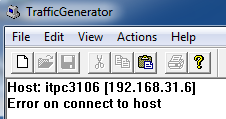
\includegraphics[width =0.4\textwidth]{connection-failed.PNG}
	\caption{Connection failed!}
	\label{user-error}
\end{figure}
%%%%%%%%%%%%%%%%%%%%%%%%%%%%%%%%%%%%%%%%%%%%%%%%%%%%%%%%%%%%%%%%%%%%%%%%%%%%%%%%%%%%%%%%%%%%%%%%%%%%%%%%%
%%%%%%%%%%%%%%%%%%%%%%%%%%%%%%%%%%%%%%%%%%%%%%%%%%%%%%%%%%%%%%%%%%%%%%%%%%%%%%%%%%%%%%%%%%%%%%%%%%%%%%%%%
%%%%%%%%%%%%%%%%%%%%%%%%%%%%%%%%%%%%%%%%%%%%%%%%%%%%%%%%%%%%%%%%%%%%%%%%%%%%%%%%%%%%%%%%%%%%%%%%%%%%%%%%%
\chapter{IPv6/ICMPv6 analysis}
\label{ipv6}
In the third and last part of the laboratory we analyzed the new versions of the protocols IPv6 and ICMPv6 using Wireshark. There are some major differences to the version 4 headers of both protocols. The first thing to notice are the much larger address segments in the headers. Those segments now support much larger address spaces to handle IPv6-addresses. 
\\\\
Table \ref{ipv6-header} shows the header for the Internet Protocol v6.
There is a new segment simply called 'Next Header' in the IP header, that handles the type of the next header. The next header usually specifies the transport layer protocol used by a packet's payload. But there can also be extension headers for IP which are specified using this field.
Also the Time to Life in the IP-header has finally been renamed to what it actually is: a Hop Limit, that is decreased when the packet bypasses a network node. 
\begin{table}[H]
	\centering
	\label{ipv6-header}
	\begin{tabular}{|c|c|c|c|c|c|c|c|c|}
		\hline
		bits       & 0-3          & 4-7             & 8-11             & 12-15      & 16-19           & 20-23          & 24-27          & 28-31         \\ \hline
		bytes      & \multicolumn{2}{c|}{0}         & \multicolumn{2}{c|}{1}        & \multicolumn{2}{c|}{2}           & \multicolumn{2}{c|}{3}         \\ \hline
		Offset 0   & Version      & \multicolumn{2}{c|}{Traffic Class} & \multicolumn{5}{c|}{Flow Label}                                                \\ \hline
		Offset 32  & \multicolumn{4}{c|}{Payload Length}                            & \multicolumn{2}{c|}{Next Header} & \multicolumn{2}{c|}{Hop Limit} \\ \hline
		Offset 64  & \multicolumn{8}{c|}{Source Address}                                                                               \\ \cline{1-1}
		Offset 96  & \multicolumn{8}{c|}{}                                                                                                              \\ \cline{1-1}
		Offset 128 & \multicolumn{8}{c|}{}                                                                                                              \\ \cline{1-1}
		Offset 160 & \multicolumn{8}{c|}{}                                                                                                              \\ \hline
		Offset 192 & \multicolumn{8}{c|}{Destination Address}                                                                         \\ \cline{1-1}
		Offset 224 & \multicolumn{8}{c|}{}                                                                                                              \\ \cline{1-1}
		Offset 256 & \multicolumn{8}{c|}{}                                                                                                              \\ \cline{1-1}
		Offset 288 & \multicolumn{8}{c|}{}                                                                                                              \\ \hline
	\end{tabular}
	\caption{Internet Protocol v6 Header}
\end{table}

Table \ref{icmpv6-header} shows the header for the Internet Control Message Protocol v6. ICMP now does the same thing ARP did in version 4. It maps IPv6 Addresses to actual MAC-Addresses using the Neighbour Discovery Protocol (NDP).

\begin{table}[H]
	\centering
	\label{icmpv6-header}
	\begin{tabular}{|c|c|c|c|c|}
		\hline
		bits      & 0-7  & 8-15 & 16-23         & 24-31         \\ \hline
		bytes     & 0    & 1    & 2             & 3             \\ \hline
		Offset 0  & Type & Code & \multicolumn{2}{c|}{Checksum} \\ \hline
		Offset 32 & \multicolumn{4}{c|}{Message Body}           \\ \hline
	\end{tabular}
	\caption{Internet Control Message Protocol v6 Header}
\end{table}

Table \ref{icmpv6-abstract-header} shows the abstract header for the Internet Control Message Protocol v6.
\begin{table}[H]
	\centering
	\label{icmpv6-abstract-header}
	\begin{tabular}{|c|c|c|c|c|}
		\hline
		bits       & 0-7        & 8-15       & 16-23       & 24-31             \\ \hline
		bytes      & 0          & 1          & 2           & 3                 \\ \hline
		Offset 0   & \multicolumn{4}{c|}{Source Address}      \\ \cline{1-1}
		Offset 32  & \multicolumn{4}{c|}{}                                     \\ \cline{1-1}
		Offset 64  & \multicolumn{4}{c|}{}                                     \\ \cline{1-1}
		Offset 96  & \multicolumn{4}{c|}{}                                     \\ \hline
		Offset 128 & \multicolumn{4}{c|}{Destination Address} \\ \cline{1-1}
		Offset 160 & \multicolumn{4}{c|}{}                                     \\ \cline{1-1}
		Offset 192 & \multicolumn{4}{c|}{}                                     \\ \cline{1-1}
		Offset 224 & \multicolumn{4}{c|}{}                                     \\ \hline
		Offset 256 & \multicolumn{4}{c|}{ICMPv6 length}                        \\ \hline
		Offset 288 & \multicolumn{3}{c|}{Zeros}            & Next Header       \\ \hline
	\end{tabular}
	\caption{Abstract Internet Control Message Protocol v6 Header}
\end{table}
\section{Node configuration}
The first task in this laboratory was the same as in laboratory 1: Checking the IP-Addresses of the PCs used in the lab to find out to whom the PING-Commands (s. chapter \ref{pingv6}) should be sent. This can be done using Window's 'ipconfig \textbackslash all'-command in the console or by using the advanced 'netsh int IPv6 show addresses'-command to show all relevant network interfaces for the PC.
\subsection{IPv4 and IPv6 configuration}
The following listing \ref{ip-config-all} shows the output for the console command 'ipconfig \textbackslash all'. Unnecessary configurations such as the configurations for IPv4 were removed for this listing:
\\ 
\begin{lstlisting}[caption={IP Config},captionpos=b,label{ip-config-all}]
Windows-IP-Konfiguration

	Hostname  . . . . . . . . . . . . : itpc3105
	Primäres DNS-Suffix . . . . . . . : rznt.rzdir.fht-esslingen.de
	Knotentyp . . . . . . . . . . . . : Hybrid
	IP-Routing aktiviert  . . . . . . : Nein
	WINS-Proxy aktiviert  . . . . . . : Nein
	DNS-Suffixsuchliste . . . . . . . : rznt.rzdir.fht-esslingen.de
									rzdir.fht-esslingen.de
									hs-esslingen.de
Ethernet-Adapter IPV6:

	Verbindungsspezifisches DNS-Suffix:
	Beschreibung. . . . . . . . . . . : Broadcom BCM5709C NetXtreme II GigE (NDISVBD Client)
	Physikalische Adresse . . . . . . : 00-0A-F7-0F-68-30
	DHCP aktiviert. . . . . . . . . . : Ja
	Autokonfiguration aktiviert . . . : Ja
	IPv6-Adresse. . . . . . . . . . . : 2001:7c0:c00:19d:518b:9700:9521:f813(Bevorzugt)
	Temporäre IPv6-Adresse. . . . . . : 2001:7c0:c00:19d:8873:ffa4:3014:bee(Bevorzugt)
	Verbindungslokale IPv6-Adresse  . : fe80::518b:9700:9521:f813%12(Bevorzugt)
	Standardgateway . . . . . . . . . : fe80::2e0:29ff:fe24:f2be%12
	DNS-Server  . . . . . . . . . . . : fec0:0:0:ffff::1%1
									fec0:0:0:ffff::2%1
									fec0:0:0:ffff::3%1
	NetBIOS über TCP/IP . . . . . . . : Deaktiviert
\end{lstlisting}
\subsection{interfaces for IPv6}
The following listing \ref{netsh-interfaces} shows the network interfaces for the Internet Protocol v6. These were displayed using the console command 'netsh int IPv6 show addresses'.
\\
\begin{lstlisting}[caption={IPv6 netsh interfaces},captionpos=b,label{netsh-interfaces}]
Schnittstelle 1: Loopback Pseudo-Interface 1

Adresstyp  DAD-Status  Gueltigkeit Bevorzugt Adresse
---------  ----------- ---------- ---------- ------------------------
Andere     Bevorzugt     infinite   infinite ::1

Schnittstelle 19: 6TO4 Adapter

Adresstyp  DAD-Status  Gueltigkeit Bevorzugt Adresse
---------  ----------- ---------- ---------- ------------------------
Andere     Bevorzugt     infinite   infinite 2002:866c:824::866c:824

Schnittstelle 11: IPV4-pub

Adresstyp  DAD-Status  Gueltigkeit Bevorzugt Adresse
---------  ----------- ---------- ---------- ------------------------
Andere     Bevorzugt     infinite   infinite fe80::8b8:182:9a03:a4fc%11

Schnittstelle 18: VirtualBox Host-Only Network

Adresstyp  DAD-Status  Gueltigkeit Bevorzugt Adresse
---------  ----------- ---------- ---------- ------------------------
Andere     Bevorzugt     infinite   infinite fe80::184e:5e69:8495:6dec%18

Schnittstelle 12: IPV6

Adresstyp  DAD-Status  Gueltigkeit Bevorzugt Adresse
---------  ----------- ---------- ---------- ------------------------
Oeffentlich Bevorzugt  29d23h59m58s 6d23h59m58s 2001:7c0:c00:19d:518b:9700:9521:f813
Temporaer   Bevorzugt  6d23h40m27s 6d23h40m27s 2001:7c0:c00:19d:8873:ffa4:3014:bee
Andere     Bevorzugt     infinite   infinite fe80::518b:9700:9521:f813%12

Schnittstelle 16: VMware Network Adapter VMnet1

Adresstyp  DAD-Status  Gueltigkeit Bevorzugt Adresse
---------  ----------- ---------- ---------- ------------------------
Andere     Bevorzugt     infinite   infinite fe80::e4fd:7474:65e0:77cc%16

Schnittstelle 17: VMware Network Adapter VMnet8

Adresstyp  DAD-Status  Gueltigkeit Bevorzugt Adresse
---------  ----------- ---------- ---------- ------------------------
Andere     Bevorzugt     infinite   infinite fe80::61f6:ca2c:cd5e:9d1e%17
\end{lstlisting}

\section{PING commands}
\label{pingv6}
For the following exercises the PING-command was used again to generate ICMP/IPv6 traffic in the network. These packets were again captured by Wireshark and analyzed to point out the differences between the new versions (v6) of these protocols compared to the older versions (v4) from the first laboratory in this workshop. The protocol stack however still stays the same. ICMPv6 request or reply packets are embedded in the IPv6 packet. And of course the IPv6 packet occupies parts of the payload segment of the Ethernet II frame (s. chapter \ref{ipv4}).
\subsection{a) Basic ICMPv6 PING command}
This PING-Command is equivalent to the very first PING-command in this workshop (s. chapter \ref{first-ping}). The only difference here is, that now ICMPv6/IPv6 is used instead of v4. The following PING-command does this:
\begin{center}
	\textit{ping -6 -n1 -l 64 2001:7c0:c00:19d:518b:9700:9521:f813}
\end{center}
Again Wireshark captured two sent packets for this PING-Command: An ICMPv6 request packet and an ICMPv6 reply packet. The size of the ICMPv6 packets however is larger than the size of the ICMPv4 packets, because the IPv6 header occupies 40 bytes instead of 20 as the IPv4 header does. This is why the ICMPv6 request packet has 126 bytes, while the ICMPv4 request packet from chapter \ref{first-ping} had only 106 bytes, although the amount of sent data is the same in both cases (64 bytes). The following listing shows the ICMPv6 request and reply packets:
\\
\begin{lstlisting}[caption={Simple ICMPv6 Ping},captionpos=b,label{icmpv5-ping}]
No.     Time           Source                Destination           Protocol Length Info
155 183.058271     2001:7c0:c00:19d:3c3d:b555:99e1:2a35 2001:7c0:c00:19d:518b:9700:9521:f813 ICMPv6   126    Echo (ping) request id=0x0001, seq=13, hop limit=128 (reply in 156)

Frame 155: 126 bytes on wire (1008 bits), 126 bytes captured (1008 bits) on interface 0
	Interface id: 0 (\\Device\\NPF\_{4B57F170-DC25-4B98-9415-3FA58C45E7F6})
		Interface name: \\Device\\NPF\_{4B57F170-DC25-4B98-9415-3FA58C45E7F6}
	Encapsulation type: Ethernet (1)
	Arrival Time: Nov 18, 2017 12:38:14.859626000 Mitteleuropäische Zeit
	[Time shift for this packet: 0.000000000 seconds]
	Epoch Time: 1511005094.859626000 seconds
	[Time delta from previous captured frame: 0.000019000 seconds]
	[Time delta from previous displayed frame: 0.000019000 seconds]
	[Time since reference or first frame: 183.058271000 seconds]
	Frame Number: 155
	Frame Length: 126 bytes (1008 bits)
	Capture Length: 126 bytes (1008 bits)
	[Frame is marked: True]
	[Frame is ignored: False]
	[Protocols in frame: eth:ethertype:ipv6:icmpv6:data]
	[Coloring Rule Name: ICMP]
	[Coloring Rule String: icmp || icmpv6]
Ethernet II, Src: Broadcom\_0f:68:28 (00:0a:f7:0f:68:28), Dst: Broadcom\_0f:68:30 (00:0a:f7:0f:68:30)
	Destination: Broadcom\_0f:68:30 (00:0a:f7:0f:68:30)
		Address: Broadcom\_0f:68:30 (00:0a:f7:0f:68:30)
		.... ..0. .... .... .... .... = LG bit: Globally unique address (factory default)
		.... ...0 .... .... .... .... = IG bit: Individual address (unicast)
	Source: Broadcom\_0f:68:28 (00:0a:f7:0f:68:28)
		Address: Broadcom\_0f:68:28 (00:0a:f7:0f:68:28)
		.... ..0. .... .... .... .... = LG bit: Globally unique address (factory default)
		.... ...0 .... .... .... .... = IG bit: Individual address (unicast)
	Type: IPv6 (0x86dd)
	Internet Protocol Version 6, Src: 2001:7c0:c00:19d:3c3d:b555:99e1:2a35, Dst: 2001:7c0:c00:19d:518b:9700:9521:f813
	0110 .... = Version: 6
		.... 0000 0000 .... .... .... .... .... = Traffic Class: 0x00 (DSCP: CS0, ECN: Not-ECT)
		.... 0000 00.. .... .... .... .... .... = Differentiated Services Codepoint: Default (0)
	.... .... ..00 .... .... .... .... .... = Explicit Congestion Notification: Not ECN-Capable Transport (0)
	.... .... .... 0000 0000 0000 0000 0000 = Flow Label: 0x00000
	Payload Length: 72
	Next Header: ICMPv6 (58)
	Hop Limit: 128
	Source: 2001:7c0:c00:19d:3c3d:b555:99e1:2a35
	Destination: 2001:7c0:c00:19d:518b:9700:9521:f813
	[Source GeoIP: Unknown]
	[Destination GeoIP: Unknown]
Internet Control Message Protocol v6
	Type: Echo (ping) request (128)
	Code: 0
	Checksum: 0x76cc [correct]
	[Checksum Status: Good]
	Identifier: 0x0001
	Sequence: 13
	[Response In: 156]
Data (64 bytes)


No.     Time           Source                Destination           Protocol Length Info
156 183.058370     2001:7c0:c00:19d:518b:9700:9521:f813 2001:7c0:c00:19d:3c3d:b555:99e1:2a35 ICMPv6   126    Echo (ping) reply id=0x0001, seq=13, hop limit=64 (request in 155)

Frame 156: 126 bytes on wire (1008 bits), 126 bytes captured (1008 bits) on interface 0
	Interface id: 0 (\\Device\\NPF\_{4B57F170-DC25-4B98-9415-3FA58C45E7F6})
		Interface name: \\Device\\NPF\_{4B57F170-DC25-4B98-9415-3FA58C45E7F6}
	Encapsulation type: Ethernet (1)
	Arrival Time: Nov 18, 2017 12:38:14.859725000 Mitteleuropäische Zeit
	[Time shift for this packet: 0.000000000 seconds]
	Epoch Time: 1511005094.859725000 seconds
	[Time delta from previous captured frame: 0.000099000 seconds]
	[Time delta from previous displayed frame: 0.000099000 seconds]
	[Time since reference or first frame: 183.058370000 seconds]
	Frame Number: 156
	Frame Length: 126 bytes (1008 bits)
	Capture Length: 126 bytes (1008 bits)
	[Frame is marked: True]
	[Frame is ignored: False]
	[Protocols in frame: eth:ethertype:ipv6:icmpv6:data]
	[Coloring Rule Name: ICMP]
	[Coloring Rule String: icmp || icmpv6]
Ethernet II, Src: Broadcom\_0f:68:30 (00:0a:f7:0f:68:30), Dst: Broadcom\_0f:68:28 (00:0a:f7:0f:68:28)
	Destination: Broadcom\_0f:68:28 (00:0a:f7:0f:68:28)
		Address: Broadcom\_0f:68:28 (00:0a:f7:0f:68:28)
		.... ..0. .... .... .... .... = LG bit: Globally unique address (factory default)
		.... ...0 .... .... .... .... = IG bit: Individual address (unicast)
	Source: Broadcom\_0f:68:30 (00:0a:f7:0f:68:30)
		Address: Broadcom\_0f:68:30 (00:0a:f7:0f:68:30)
		.... ..0. .... .... .... .... = LG bit: Globally unique address (factory default)
		.... ...0 .... .... .... .... = IG bit: Individual address (unicast)
Type: IPv6 (0x86dd)
	Internet Protocol Version 6, Src: 2001:7c0:c00:19d:518b:9700:9521:f813, Dst: 2001:7c0:c00:19d:3c3d:b555:99e1:2a35
	0110 .... = Version: 6
		.... 0000 0000 .... .... .... .... .... = Traffic Class: 0x00 (DSCP: CS0, ECN: Not-ECT)
		.... 0000 00.. .... .... .... .... .... = Differentiated Services Codepoint: Default (0)
	.... .... ..00 .... .... .... .... .... = Explicit Congestion Notification: Not ECN-Capable Transport (0)
	.... .... .... 0000 0000 0000 0000 0000 = Flow Label: 0x00000
	Payload Length: 72
	Next Header: ICMPv6 (58)
	Hop Limit: 64
	Source: 2001:7c0:c00:19d:518b:9700:9521:f813
	Destination: 2001:7c0:c00:19d:3c3d:b555:99e1:2a35
	[Source GeoIP: Unknown]
	[Destination GeoIP: Unknown]
Internet Control Message Protocol v6
	Type: Echo (ping) reply (129)
	Code: 0
	Checksum: 0x75cc [correct]
	[Checksum Status: Good]
	Identifier: 0x0001
	Sequence: 13
	[Response To: 155]
	[Response Time: 0.099 ms]
Data (64 bytes)
\end{lstlisting}
\subsection{b) ICMPv6 PING command with large data package}
For this exercise another PING-Command was used to send a large data packet from one PC to another. The data field of this packet was large enough to enforce fragmentation.
\begin{center}
	\textit{ping -6 -n1 -l 2000 2001:7c0:c00:19d:518b:9700:9521:f813}
\end{center}
As the maximal size of an Ethernet frame is 1510 bytes, this large amount of data must be fragmented into two separate packets by IPv6. As seen in chapter \ref{ipv4} the Ethernet II segments occupy 14 bytes of data. Having a look on the introduction of this laboratory (s. chapter \ref{ipv6}), one can see that the ICMPv6 header still only occupies 8 bytes. But the IPv6 header now has a size of 40 bytes and the packet must must also contain information about the fragmentation in an additional fragmentation header (another 8 bytes) as routers cannot fragment IPv6 packets. Subtracting these segments from the Ethernet frame's maximal size determines the MTU for one IPv6 fragment:
\begin{center}
	MTU = 1510 bytes -14 bytes -8 bytes -40 bytes -8 bytes
		= \underline{1440 bytes} 
\end{center} 
This first data packet is sent using an IPv6 packet with an IP fragmentation header and contains the first 1440 bytes of transmitted data. The second packet that is immediately sent after the IPv6 fragment is a ICMPv6 request packet containing the remaining 560 bytes of data, the ICMPv6 header (8 bytes), the IPv6 header (40 bytes) , and the Ethernet segments (14 bytes). So summed up this second packet has a size of 622 bytes. The reply packets are fragmented the same way. The following Wireshark trace shows all four collapsed packets transmitted between both PCs.
\\
\begin{lstlisting}[caption={IPv6 Fragmentation},captionpos=b,label{icmpv6-ping-fragment}]
No.     Time           Source                Destination           Protocol Length Info
9 1.250164       2001:7c0:c00:19d:3c3d:b555:99e1:2a35 2001:7c0:c00:19d:518b:9700:9521:f813 IPv6     1510   IPv6 fragment (off=0 more=y ident=0x00000000 nxt=58)

Frame 9: 1510 bytes on wire (12080 bits), 1510 bytes captured (12080 bits) on interface 0
Ethernet II, Src: Broadcom\_0f:68:28 (00:0a:f7:0f:68:28), Dst: Broadcom\_0f:68:30 (00:0a:f7:0f:68:30)
Internet Protocol Version 6, Src: 2001:7c0:c00:19d:3c3d:b555:99e1:2a35, Dst: 2001:7c0:c00:19d:518b:9700:9521:f813
Data (1448 bytes)

No.     Time           Source                Destination           Protocol Length Info
10 1.250167       2001:7c0:c00:19d:3c3d:b555:99e1:2a35 2001:7c0:c00:19d:518b:9700:9521:f813 ICMPv6   622    Echo (ping) request id=0x0001, seq=14, hop limit=128 (reply in 13)

Frame 10: 622 bytes on wire (4976 bits), 622 bytes captured (4976 bits) on interface 0
Ethernet II, Src: Broadcom\_0f:68:28 (00:0a:f7:0f:68:28), Dst: Broadcom\_0f:68:30 (00:0a:f7:0f:68:30)
Internet Protocol Version 6, Src: 2001:7c0:c00:19d:3c3d:b555:99e1:2a35, Dst: 2001:7c0:c00:19d:518b:9700:9521:f813
Internet Control Message Protocol v6

No.     Time           Source                Destination           Protocol Length Info
12 1.250367       2001:7c0:c00:19d:518b:9700:9521:f813 2001:7c0:c00:19d:3c3d:b555:99e1:2a35 IPv6     1510   IPv6 fragment (off=0 more=y ident=0x00000000 nxt=58)

Frame 12: 1510 bytes on wire (12080 bits), 1510 bytes captured (12080 bits) on interface 0
Ethernet II, Src: Broadcom\_0f:68:30 (00:0a:f7:0f:68:30), Dst: Broadcom\_0f:68:28 (00:0a:f7:0f:68:28)
Internet Protocol Version 6, Src: 2001:7c0:c00:19d:518b:9700:9521:f813, Dst: 2001:7c0:c00:19d:3c3d:b555:99e1:2a35
Data (1448 bytes)

No.     Time           Source                Destination           Protocol Length Info
13 1.250368       2001:7c0:c00:19d:518b:9700:9521:f813 2001:7c0:c00:19d:3c3d:b555:99e1:2a35 ICMPv6   622    Echo (ping) reply id=0x0001, seq=14, hop limit=64 (request in 10)

Frame 13: 622 bytes on wire (4976 bits), 622 bytes captured (4976 bits) on interface 0
Ethernet II, Src: Broadcom\_0f:68:30 (00:0a:f7:0f:68:30), Dst: Broadcom\_0f:68:28 (00:0a:f7:0f:68:28)
Internet Protocol Version 6, Src: 2001:7c0:c00:19d:518b:9700:9521:f813, Dst: 2001:7c0:c00:19d:3c3d:b555:99e1:2a35
Internet Control Message Protocol v6
\end{lstlisting}
\subsection{c) Rebooting PC}
For this exercise the PC from where the previous PING-Commands were executed was shut down and rebooted, while the network activity was observed using the second PC. The aim was to get an idea of the Neighbor Discovery Protocol (NDP) and the Stateless Address Auto Configuration (SLAAC), that replace the Address Resolution Protocol (ARP) in IPv6.
\subsection{d) Enforcing Neighbor discovery}
\subsection{e) ICMPv6 PING command with destination in another subnet}
\subsection{f) PING to a remote tunnel end}

%%%%%%%%%%%%%%%%%%%%%%%%%%%%%%%%%%%%%%%%%%%%%%%%%%%%%%%%%%%%%%%%%%%%%%%%%%%%%%%%%%%%%%%%%%%%%%%%%%%%%%%%%
%%%%%%%%%%%%%%%%%%%%%%%%%%%%%%%%%%%%%%%%%%%%%%%%%%%%%%%%%%%%%%%%%%%%%%%%%%%%%%%%%%%%%%%%%%%%%%%%%%%%%%%%%
%%%%%%%%%%%%%%%%%%%%%%%%%%%%%%%%%%%%%%%%%%%%%%%%%%%%%%%%%%%%%%%%%%%%%%%%%%%%%%%%%%%%%%%%%%%%%%%%%%%%%%%%%
\chapter{Conclusion}
\label{conclusion}